% !TeX program = pdflatex
\documentclass[11pt]{article}
\usepackage[margin=1in]{geometry}
\usepackage{enumitem}
\usepackage{xcolor}
\usepackage{hyperref}
\usepackage{cite}
\usepackage{setspace}
\usepackage{amsmath}
\usepackage{amssymb}
\usepackage{multirow}
\usepackage{graphicx}
\usepackage{booktabs}
\usepackage{caption}
\captionsetup{
    labelfont={color=blue},
    textfont={color=blue}
}
\setlength{\parskip}{6pt}
\setlength{\parindent}{0pt}
\setlist[enumerate]{leftmargin=0pt,labelindent=0pt,itemindent=0pt,listparindent=0pt,label={},labelsep=0pt,align=left,itemsep=0.5em}
\newcommand{\reviewersection}[1]{\section*{Reviewer~#1}}
\newcommand{\commentresponse}[2]{{\color{blue}\textbf{Response:} #2}}
\newcommand{\commentitem}{\item \textbf{Comment~\arabic{enumi}.}\\\ignorespaces}

\begin{document}

\begin{center}
    {\Large\bfseries Response to Reviewers}

    {\normalsize Title: SMC-Net: Structure-Aware Multi-Scale Coarse-to-Fine Cascaded Network for Joint Choroid Layer and Vessel Segmentation}
\end{center}

Dear Editor and Reviewers,\\
We would like to sincerely thank you for the time and effort devoted to the review of our previously submitted manuscript entitled
``SMC-Net: Structure-Aware Multi-Scale Coarse-to-Fine Cascaded Network for Joint Choroid Layer and Vessel Segmentation''
(Manuscript ID: MM-024752).
We greatly appreciate the detailed and constructive comments, which have provided valuable guidance for improving this work.

Motivated by your feedback, we have carefully re-examined the problem formulation and conducted a thorough and substantial revision of the manuscript.
The revised version reflects significant improvements in the proposed methodology, experimental validation, and technical clarity, together with a clearer and more focused presentation of the paper’s contributions.
We now submit this revised work as a new manuscript.

Compared with the previous version, the main revisions include:
\begin{itemize}
    \item \textbf{Manuscript restructuring and consolidation:} We have reorganized the paper to improve clarity and self-containedness, integrating essential analyses, ablation studies, and implementation details directly into the main manuscript.
    \item \textbf{Expanded comparisons and ablations:} We have added new experiments to address major concerns raised in the previous review, including comparisons between SSSD and VSSD, and between UPED and multi-directional Sobel as well as other edge-detection baselines, together with expanded quantitative and qualitative analyses.
    \item \textbf{Stronger methodological clarification:} We have substantially strengthened the technical explanations and justifications of the proposed modules, problem formulation, and design choices, and clarified the applicability and limitations of relevant baselines.
    \item \textbf{Improved presentation and readability:} We have revised the abstract, figures, and tables, and refined the writing throughout the manuscript to improve clarity and coherence.
\end{itemize}

In the following sections, we provide a detailed, point-by-point response to all comments raised in the previous round of reviews.
All newly added or modified text is highlighted in {\color{red}red} within the revised manuscript for ease of verification.
For convenience, cited text from the manuscript is shown in {\color{blue}blue} italics in this response letter.

Sincerely,\\
Yang Wen, Shunzhe Shen, Lei Bi, Wuzhen Shi, Ping Li, Bin Sheng, and Xiaokang Yang

\reviewersection{1}
Recommendation: AQ - Publish With Minor, Required Changes
\begin{enumerate}
    \commentitem It is suggested that the abstract be further shortened and the key content be retained to make the abstract more concise. It is also suggested that the specific experimental results be placed in the abstract to make it a directly readable paragraph.
    
    \commentresponse{1}{
    Thank you for this constructive suggestion. 
    We have streamlined the abstract and made the main contributions and experimental advantages more immediately clear. Specifically, we have (1) condensed the description of challenges posed by noisy OCT and cascaded error propagation in a single sentence, (2) reframed the method description into a concise SMC-Net sentence centred on the SSSD-based coarse-to-fine design, and (3) added a comparative performance summary that highlights our improvements over the strongest choroid-specific baseline (TACLNet) on RETOUCH dataset. The revised abstract is highlighted in red in the revised manuscript. For convenience, we also reproduce the full revised abstract below in blue italics:\\
    \\
    \textit{{\color{blue}
    ``Choroid thickness and choroidal vessel index are crucial biomarkers for the diagnosis, prediction, and treatment of various ophthalmic diseases. 
    However, high-noise OCT images hamper global structural modeling, leading to inconsistent vessel topology and morphology. Furthermore, existing cascaded frameworks often propagate errors by treating choroid layers and vessels in separate stages, neglecting their inherent anatomical relationships.
    To address these challenges, we propose SMC-Net, a structure-aware multi-scale coarse-to-fine cascaded network that employs Spatiocanal State Space Duality blocks to efficiently capture global spatial and channel-wise context for joint choroid layer and vessel segmentation.
    In the coarse stage, a Mamba-based U-shaped network is employed to segment the choroidal layer to provide a reliable prior for subsequent refinement.
    In the refinement stage, a fractional-differential-based unsupervised prior extractor and Structure-Aware Modules are proposed to enhance subtle vascular structures in noisy OCT images.
    Meanwhile, a structure-aware dual-branch network jointly models choroidal layer and vessel features to explicitly capture their anatomical relationships.
    Finally, a choroidal edge-constrained joint loss is designed to enforce anatomical consistency between vessel and layer boundaries.
    Extensive experiments on the private OCT-CCV dataset and the public RETOUCH dataset demonstrate the state-of-the-art performance and robust generalization of SMC-Net. Compared with the strongest choroid-specific baseline TACLNet under comparable computational cost, our SMC-Net-S improves fluid mIoU/DSC by 2.60\%/1.75\% on RETOUCH. Code will be available.''}}
    }

    \commentitem For private datasets, it is recommended to provide specific collection processes, including data sources (which hospital), patient information, collection time intervals, and whether ethical reviews have been passed. This specific information needs to be included in the data introduction section of the article.
    
    \commentresponse{2}{
    We thank the reviewer for this important suggestion.
    We have substantially expanded the description of the private OCT-CCV dataset in Section~IV-A (Dataset) of the revised manuscript.
    The revised text now explicitly includes the data source (hospital information), patient cohort description, acquisition time span, imaging protocol, and ethical approval details.
    Specifically, we clarify that all OCT images were collected retrospectively under institutional review board (IRB) approval, with informed consent obtained where applicable, and that the study complies with relevant ethical guidelines.
    These additions ensure transparency, reproducibility, and compliance with ethical standards for clinical data usage.

    For convenience and ease of verification, we reproduce the full revised OCT-CCV dataset description below in blue italics:\\
    \\
    \textit{{\color{blue}``\textbf{OCT Clinical Choroidal Vessel Dataset (OCT-CCV).} {All OCT-CCV images used in this study were retrospectively collected at Shanghai General Hospital, Shanghai Jiao Tong University, between 2023 and 2024. The data collection was conducted under the approval of the institutional review board and in accordance with the Declaration of Helsinki. Informed consent was waived due to the retrospective study design and use of anonymized
    data.} This dataset consists of 120 images collected by experienced ophthalmologists using swept-source OCT. Each image is averaged from 32 overlapping scans centered on the fovea, with a resolution of 1024$\times$992. Ten subjects (five emmetropic and five highly myopic, $\leqslant$ -5.0) were randomly selected. Two ophthalmologists independently annotated the choroid layer and vessels, followed by joint verification. We use 5-fold cross-validation for evaluation: in each fold, eight studies (96 images, $\sim$8,740 annotated regions, resized to 512$\times$512) form the training set, while the remaining two studies (24 images, $\sim$2,190 regions) form the test set.
    ''}}
    }

    \commentitem It is recommended that the second formula in Formula 9 be displayed in separate lines to keep it within the page range.
    
    \commentresponse{3}{
    Thank you for pointing out this typesetting issue.
    In the revised manuscript, we have restructured and simplified the AMG-FFN formulation to improve clarity and conciseness.
    Specifically, the original expanded expression in Equation~(9)(Equation~(7) in the revised manuscript) has been replaced with a compact and abstracted formulation that summarizes the multi-scale depth-wise convolutions and adaptive gating mechanism in a single line.
    As a result, the revised equation naturally fits within the page margins without requiring line splitting, while preserving the original computational meaning of AMG-FFN.
    For convenience and ease of verification, we reproduce the full revised part description below in blue italics:\\
    \\
    \textit{{\color{blue}``\textbf{(b) AMG-FFN:} The Adaptive Multi-scale Gated Feed-Forward Network (AMG-FFN) is designed to enhance local feature modeling following the SSSD layer.
    Given an input feature map $h$, AMG-FFN extracts multi-scale local features using depth-wise convolutions with different kernel sizes and adaptively fuses them through a gating mechanism:
    \begin{equation}
    z = \mathcal{F}_{\text{linear}}\big(h \circ \mathcal{G}(\mathcal{F}_{\text{ms}}(h))\big)\tag{7},
    \end{equation}
    where $\mathcal{F}_{\text{ms}}(\cdot)$ denotes multi-scale depth-wise convolutional feature extraction, $\mathcal{G}(\cdot)$ represents adaptive gating, and $\circ$ is element-wise multiplication.
    This design enables AMG-FFN to selectively enhance fine-grained choroidal structures while maintaining computational efficiency.''
    }}
}

    \commentitem The current form lacks a comparative discussion on the efficiency of the models. It is recommended to add the comparison of the parameter quantity and GFLOPs of the comparison model and the proposed model in Tables 1 and 2.

    \commentresponse{4}{
    {\color{blue}
    We thank the reviewer for this valuable suggestion regarding model efficiency comparison.
    To directly address this concern, we have added explicit comparisons of parameter counts and GFLOPs between the proposed SMC-Net and all competing methods under a unified experimental setting.
    
    Specifically, we now report the number of parameters and GFLOPs for each model at an input resolution of $512\times512$, and analyze their accuracy--efficiency trade-offs.
    As shown in Fig.~7, the results show that SMC-Net achieves superior segmentation performance with substantially lower computational cost than Transformer-based baselines.
    In particular, SMC-Net-S reaches the best balance point, achieving higher vessel and layer DSC with approximately half the parameters and nearly one order of magnitude fewer GFLOPs than TACLNet, while further scaling yields diminishing performance gains.
    
    In addition, we provide an inference-time breakdown for the SMC-Net series, demonstrating that SMC-Net-S processes a $512\times512$ OCT image in 12.6~ms (79 FPS) on a single RTX~4090~D GPU, confirming its practical efficiency.
    \begin{table}[h]
    \renewcommand{\arraystretch}{1.15}
    \centering
    \begingroup\color{blue}\small
    \setlength{\tabcolsep}{4pt}
    \captionsetup[table]{name=Table III.}{Table III: Inference-time breakdown of the SMC-Net series on OCT-CCV ($512\times512$, fp32, batch=1) with an RTX 4090 D. SMC-Net-S is measured; SMC-Net-T/B are estimated by scaling the measured network time (coarse+refine) linearly with GFLOPs while keeping UPED fixed at $0.8$~ms.}
    \label{tab:inference_time_smcnet}
    \resizebox{0.7\linewidth}{!}{
    \begin{tabular}{@{}lcccccc@{}}
    \toprule
    Variant & Params (M) & GFLOPs (G) & UPED (ms) & Coarse+Refine (ms) & Total (ms) & FPS \\ \midrule
    SMC-Net-T & 11.14 & 17.60 & 0.8 & 3.1 & 3.9 & 257 \\
    SMC-Net-S & 49.04 & 67.18 & 0.8 & 11.8 & 12.6 & 79 \\
    SMC-Net-B & 72.89 & 195.73 & 0.8 & 34.4 & 35.2 & 28 \\ \bottomrule
    \end{tabular}
    }
    \endgroup
    \end{table}
    \setcounter{figure}{6}
    \begin{figure}[h]
    \centering
    \begingroup\color{blue}
    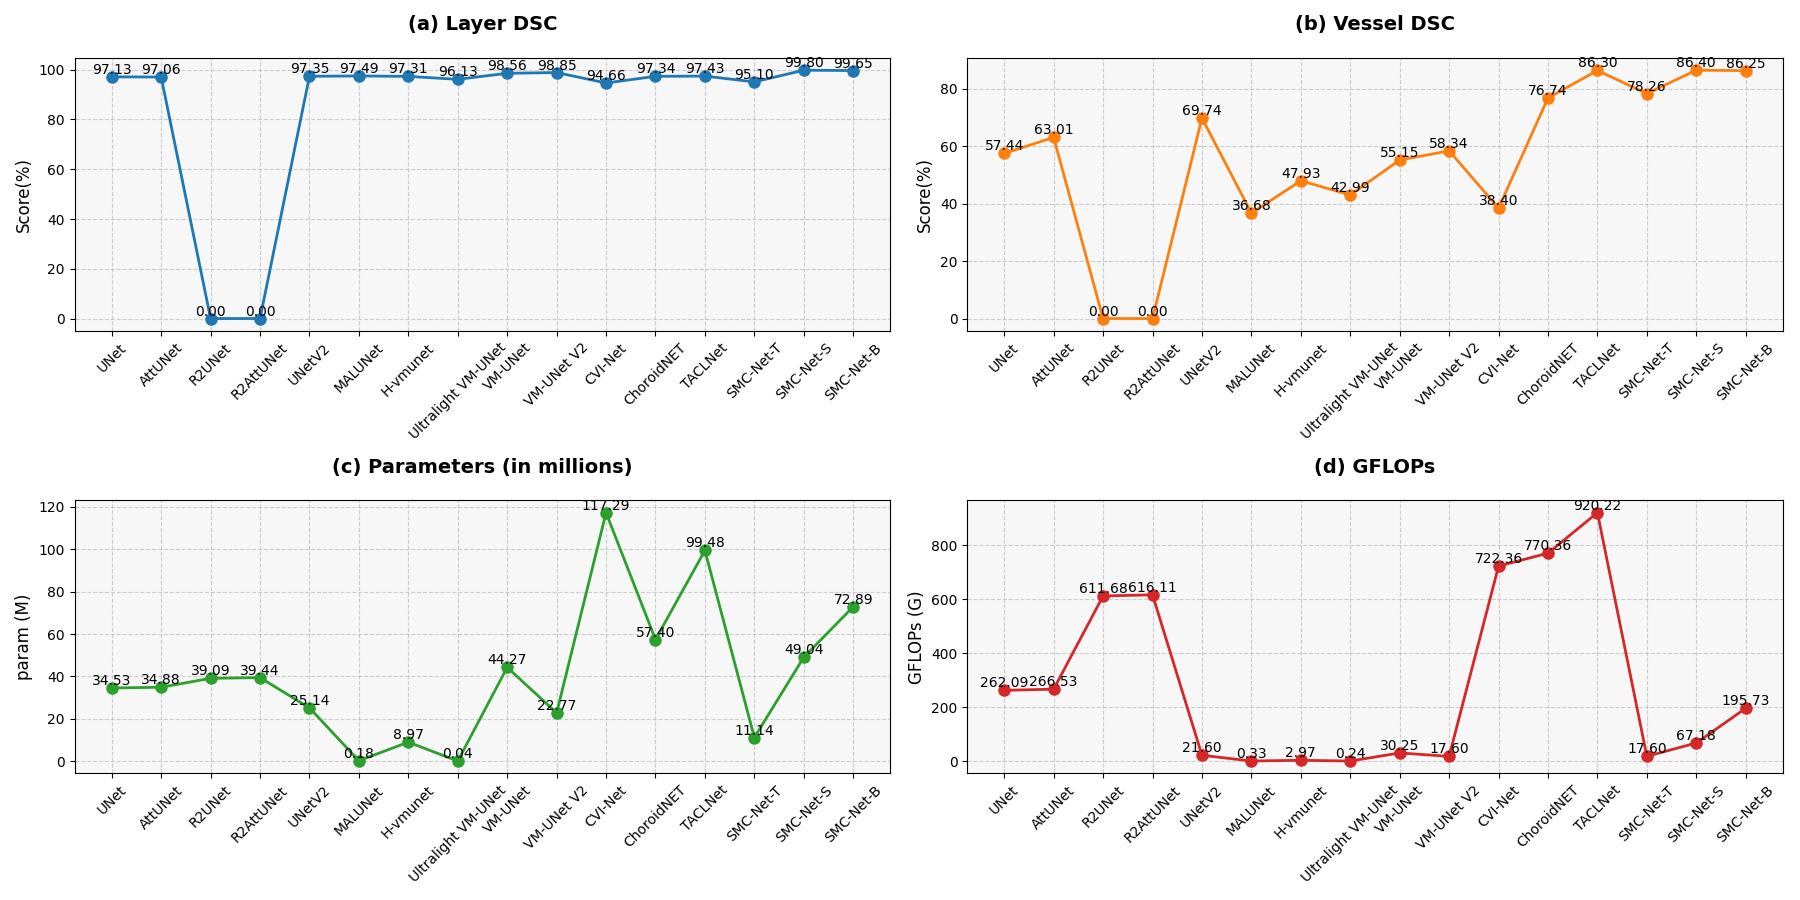
\includegraphics[width=1\linewidth]{fig/complexity_compare.png}
    \caption{Accuracy--efficiency trade-off on OCT-CCV ($512\times512$, batch=1, fp32). (a) Layer DSC, (b) Vessel DSC, (c) Params (M), (d) GFLOPs (G).}
    \label{fig:complexity_compare}
    \endgroup
    \end{figure}\\
    For completeness and ease of verification, the newly added table, figure, and corresponding discussion in the revised manuscript are quoted below: \\
    }
    \\
    \textit{{\color{blue}``\textbf{A. Scaling Trends of Computational Complexity and Performance}\\
    \textbf{1) Architecture and FLOPs Scaling}\\
    In addition to segmentation accuracy, we compare model complexity in terms of parameter count and GFLOPs on the OCT-CCV dataset.
    As shown in Fig.~\ref{fig:complexity_compare}, the proposed SMC-Net series consistently achieves a favorable accuracy--efficiency trade-off.
    In particular, SMC-Net-S attains the best choroidal layer and vessel DSC while maintaining moderate model size and computational cost.
    Compared with the Transformer-based TACLNet~\cite{wen2024}, SMC-Net-S achieves comparable or better performance with approximately half the parameters and nearly one order of magnitude fewer GFLOPs.
    Moreover, performance gains saturate beyond SMC-Net-S (49.04M parameters), indicating diminishing returns from further model scaling.\\
    \textbf{2) Inference Time}\\
    We further evaluate inference efficiency on a single NVIDIA RTX 4090 D GPU (batch size 1, $512\times512$, fp32).
    SMC-Net-S processes one OCT image in 12.6~ms (approximately 79 FPS), demonstrating its suitability for real-time or near-real-time deployment. Table III reports the inference-time breakdown of the SMC-Net series, showing consistent scaling behavior across Tiny, Small, and Base variants.''}}   
    }

    \commentitem It is suggested to add a discussion section that includes discussions on the possible clinical impacts and applications of the methods proposed in this article. Meanwhile, the discussion section contains a paragraph discussing the limitations of the method proposed in this paper.
    
    \commentresponse{5}{
    We thank the reviewer for this constructive suggestion. In response, we have added a dedicated Discussion section (Section~VI) that explicitly addresses both the potential clinical impact and the limitations of the proposed method.

    Specifically, the Discussion outlines how accurate joint segmentation of choroidal layers and vessels in swept-source OCT can support quantitative analysis relevant to myopia, age-related macular degeneration, and other chorioretinal diseases, as well as longitudinal monitoring and treatment response evaluation. In addition, we include a concise paragraph discussing current limitations of SMC-Net, including its focus on 2D B-scans and potential performance degradation under extremely poor image quality or unseen acquisition conditions, together with directions for future improvement. This addition directly follows the reviewer’s recommendation.
    The added and revised text is highlighted in the conclusion of the revised manuscript and are quoted below:\\
    \textit{{\color{blue}``\textbf{Disscussion.}\\
    Clinically, accurate joint segmentation of choroidal layers and vessels in swept-source OCT enables quantitative analysis of choroidal thickness and vascular indices, which are relevant to diseases such as myopia and age-related macular degeneration. By producing layer-aware vessel maps that are robust to noise and artifacts, SMC-Net may support longitudinal analysis and treatment response evaluation, and can serve as a preprocessing module for downstream clinical applications. Despite these advantages, the current method is limited to 2D B-scans and may degrade under extremely poor image quality or unseen acquisition conditions. Future work will explore volumetric modeling and improved robustness across devices and datasets.''}}
    }
\end{enumerate}

\reviewersection{2}
Recommendation: R - Reject
\begin{enumerate}
    \commentitem The Spatiocanal State Space Duality (SSSD) module proposed in the paper can be considered a variant of the VSSD module in reference [19]. Therefore, what advantages does the SSSD module have compared to VSSD? Please supplement comparative experiments with VSSD and conduct an analysis.
    
    \commentresponse{1}{
    Thank you for this important comment.
    We agree that a direct comparison between the proposed Spatiocanal State Space Duality (SSSD) and the Vision State Space Duality (VSSD) module is necessary to clarify their respective advantages.

    To verify the effectiveness of SSSD, we conducted head-to-head comparative experiments by replacing all SSSD blocks in SMC-Net-T/S/B with the VSSD block proposed in~\cite{shi2024vssdvisionmambanoncausal}, while keeping the rest of the architecture unchanged.
    The quantitative comparison in terms of parameters, GFLOPs, mIoU, and DSC is now reported and analyzed in Sec.V-D (\emph{Comparison between SSSD and VSSD}) of the revised manuscript.

    As shown in Table V of the revised manuscript, replacing SSSD with VSSD consistently reduces segmentation accuracy across all model scales, despite its lower computational cost.
    For example, on SMC-Net-S, VSSD results in decreases of 1.37\% mIoU and 1.38\% DSC.
    These results demonstrate that, while VSSD performs spatial-only dualization, our SSSD’s joint modeling of spatial and channel-wise dependencies better captures layer--vessel co-variation in choroidal OCT images, leading to more accurate segmentation under noisy conditions.
    \begin{table}[h]
    % \renewcommand{\arraystretch}{1.15}
    \centering
    \begingroup\color{blue}
    \captionsetup[table]{name=Table V.}{Table V: SSSD vs. VSSD comparison on OCT-CCV dataset (SMC-Net-T/S/B, vessel segmentation target).}\\
    \label{tab:sssd_vssd}
    \resizebox{0.6\linewidth}{!}{
    \begin{tabular}{lllll}
    \toprule
    Backbone & Params (M) & GFLOPs (G) & mIoU (\%) $\uparrow$ & DSC (\%) $\uparrow$ \\ \midrule
    SMC-Net-T w/ VSSD~\cite{shi2024vssdvisionmambanoncausal} & 6.96 & 11.00 & 71.82 & 82.74 \\
    SMC-Net-T (SSSD, Ours) & 11.14 & 17.60 & \textbf{73.10} & \textbf{84.12} \\ \midrule
    SMC-Net-S w/ VSSD~\cite{shi2024vssdvisionmambanoncausal} & 30.65 & 41.99 & 74.21 & 85.02 \\
    SMC-Net-S (SSSD, Ours) & 49.04 & 67.18 & \textbf{75.58} & \textbf{86.40} \\ \midrule
    SMC-Net-B w/ VSSD~\cite{shi2024vssdvisionmambanoncausal} & 45.56 & 122.33 & 74.64 & 85.41 \\
    SMC-Net-B (SSSD, Ours) & 72.89 & 195.73 & \textbf{76.02} & \textbf{86.78} \\ \bottomrule
    \end{tabular}
    }
    \endgroup
    \end{table}\\
    The revised Sec.V-D in the latest manuscript is as follows:\\
    \textit{{\color{blue}``To evaluate the benefit of the proposed Spatiocanal State Space Duality (SSSD) over the Vision State Space Duality (VSSD) block~\cite{shi2024vssdvisionmambanoncausal}, we replace all SSSD blocks in SMC-Net-T/S/B with VSSD while keeping other components unchanged.
    Table V reports the corresponding parameters, GFLOPs, mIoU, and DSC on the OCT-CCV dataset.
    Across all model scales, SSSD consistently achieves higher segmentation accuracy at the cost of increased model complexity.
    For example, on SMC-Net-S, replacing SSSD with VSSD results in performance drops of 1.37\% mIoU and 1.38\% DSC, while reducing parameters and GFLOPs by approximately 1.6$\times$.
    These results indicate that jointly modeling spatial and channel-wise dependencies enables SSSD to better capture layer--vessel co-variation in choroidal OCT images than the spatial-only VSSD design, thereby justifying its higher computational cost.''}}\\
    }

    \commentitem The unsupervised prior edge detector (UPED) algorithm proposed in the paper is designed based on the multi-directional Sobel operators edge enhancement module from literature [8]. Please supplement comparative experiments with literature [8] and conduct an analysis.
    
    \commentresponse{2}{
    Thank you for this important comment.
    We agree that a direct comparison with the multi-directional Sobel edge enhancement module proposed in~\cite{dual_encoder_edge} is necessary to clarify the advantages of the proposed Unsupervised Prior Edge Detector (UPED).

    In response, we have conducted explicit comparative experiments by integrating the multi-directional Sobel operator from~\cite{dual_encoder_edge} into our framework under the same experimental setting as UPED.
    The comparative results are now reported and analyzed in Sec.V-B (\emph{Effectiveness of the Unsupervised Prior Edge Detector}) of the revised manuscript.

    As shown in Table IV of the revised manuscript, the multi-directional Sobel baseline achieves 73.12\% mIoU and 83.65\% DSC, outperforming classical Sobel and Canny operators.
    In contrast, the proposed UPED yields further improvements, reaching 75.58\% mIoU and 86.40\% DSC, while maintaining comparable Acc, Spe, and Sen. As shown in Table VI (Rows 1--2) of the revised manuscript, introducing UPED consistently improves segmentation performance, yielding gains of 2.29\% in mIoU, 1.61\% in DSC, 0.22\% in Acc, 0.17\% in Spe, and 1.40\% in Sen. The decoder attention visualizations in Fig.~\ref{fig:ablation_decoder_attn} further indicate that UPED guides the network to focus on vascular regions rather than the entire choroid, facilitating more discriminative vessel segmentation.

    The accompanying analysis demonstrates that, compared with the integer-order multi-directional Sobel operator, UPED’s fractional-differential formulation is more effective at preserving weak vascular structures and suppressing noise in OCT images, resulting in more informative structural priors for choroidal vessel segmentation.\\
    \setcounter{figure}{7}
    \begin{figure}[h!]
    \centering
    \begingroup\color{blue}
    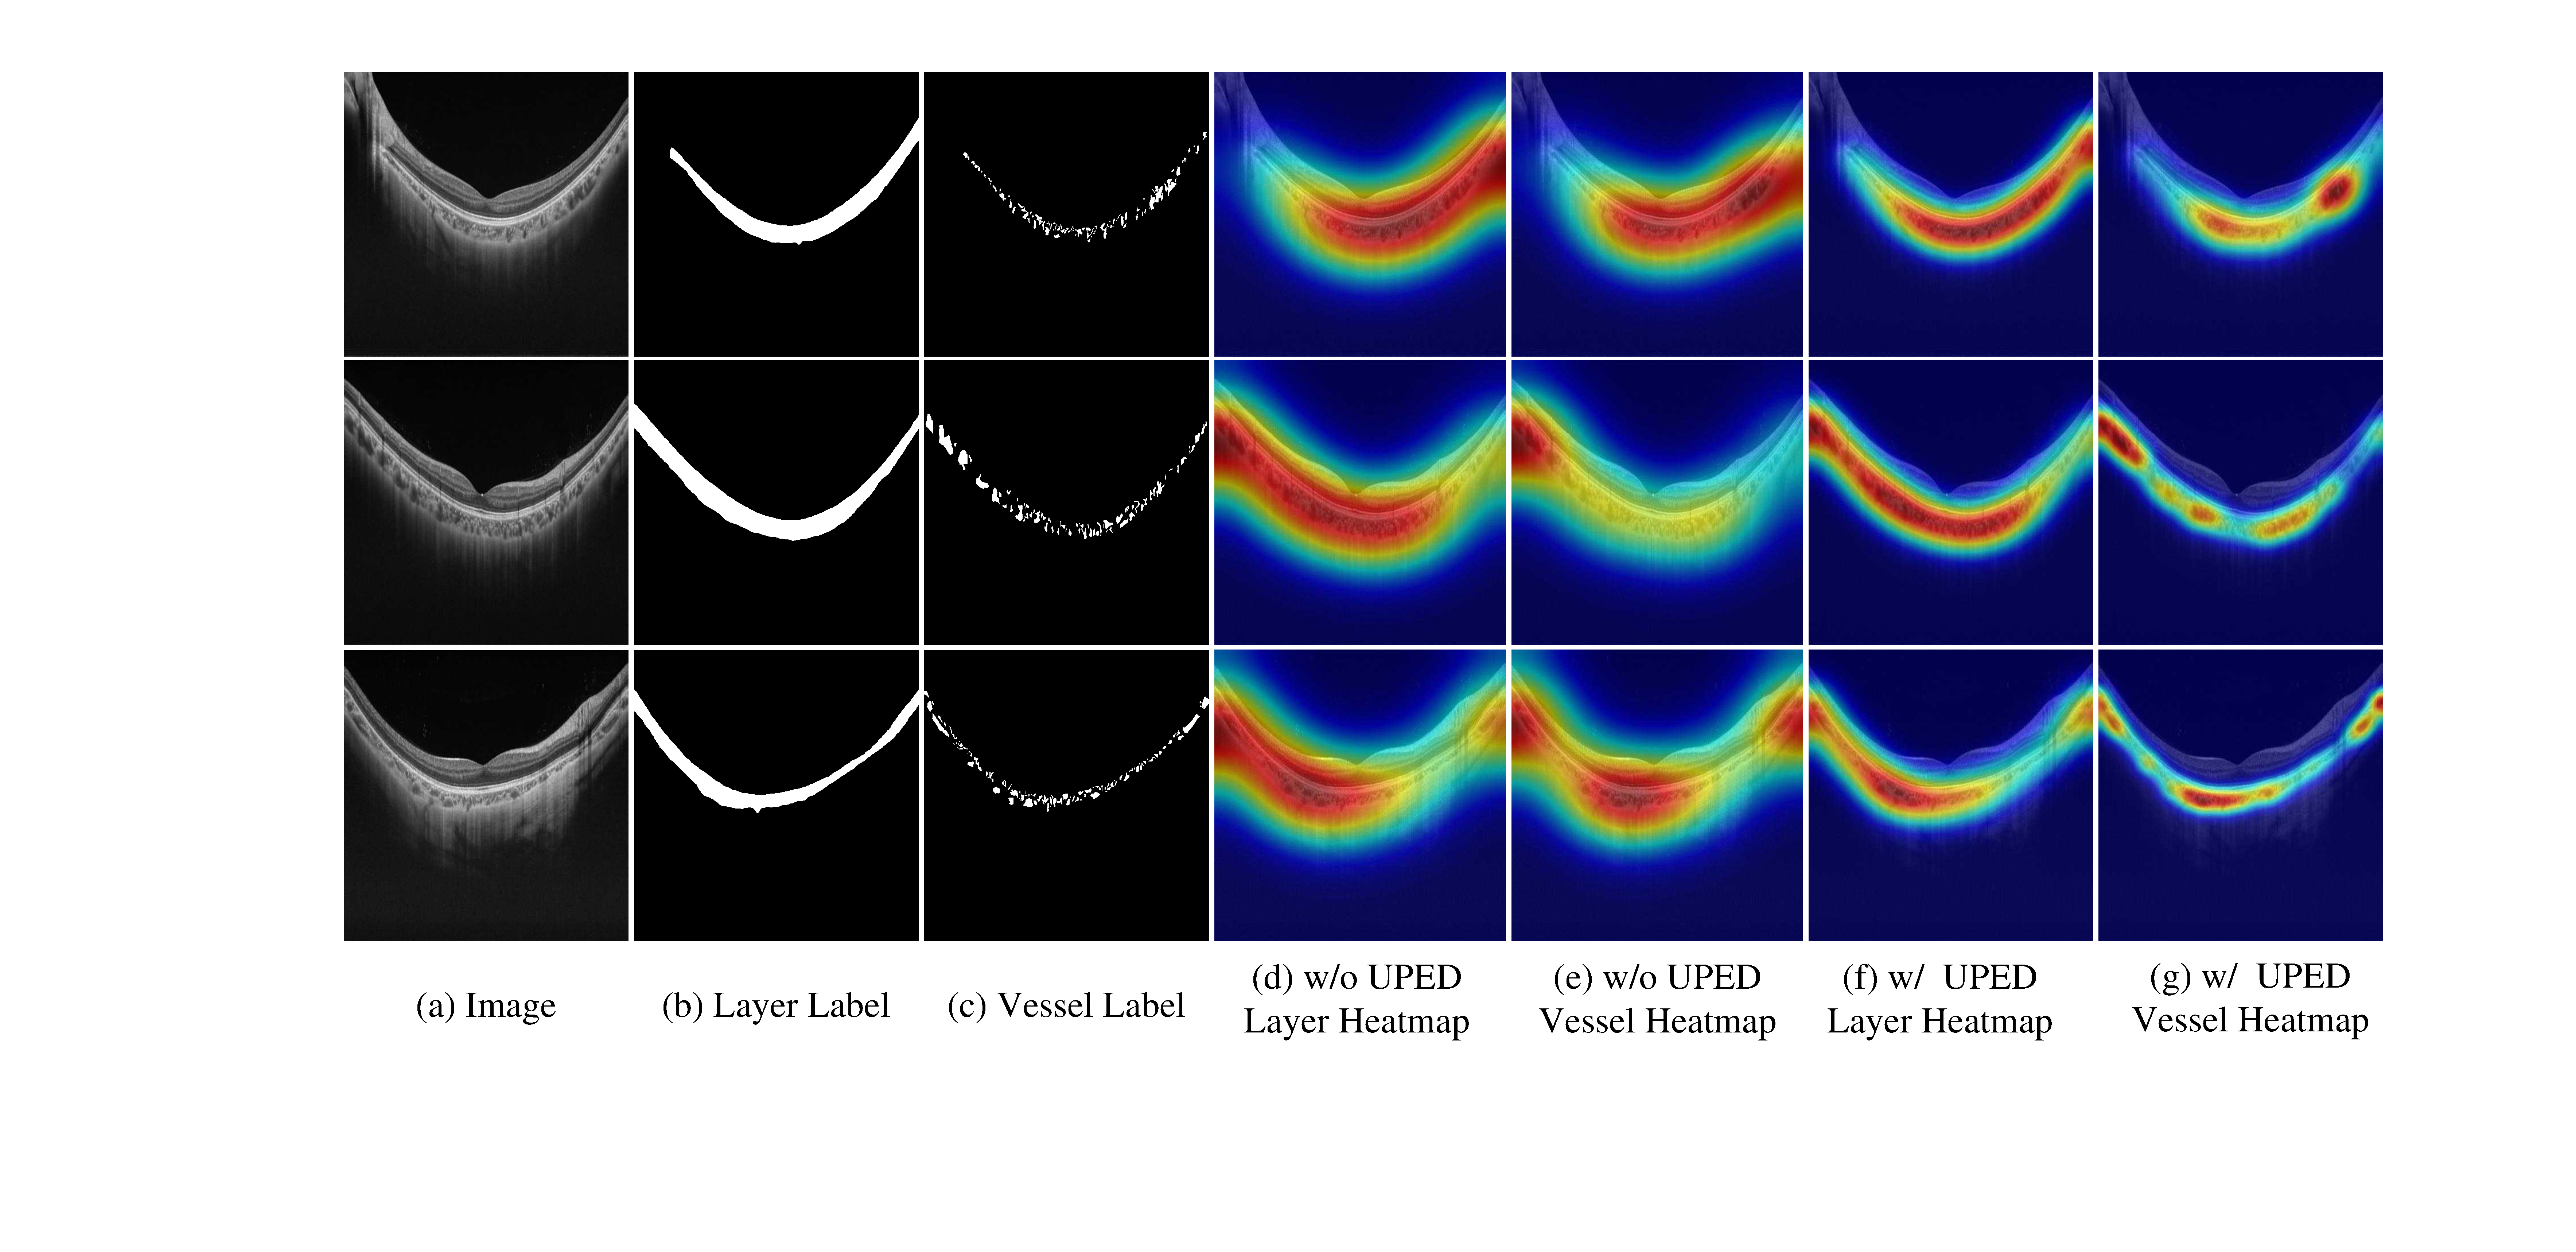
\includegraphics[width=0.6\linewidth]{fig/ablation_2.pdf}
    \caption{Visualization of decoder attention with and without UPED.
    (a) Input image, (b) choroidal layer ground truth, (c) vessel ground truth,
    (d) attention map of the layer decoder without UPED,
    (e) attention map of the vessel decoder without UPED,
    (f) attention map of the layer decoder with UPED,
    and (g) attention map of the vessel decoder with UPED.
    UPED enhances decoder focus on complex vascular regions, leading to more informative and structure-aware representations.}
    \label{fig:ablation_decoder_attn}
    \endgroup
    \end{figure}
\begin{table}[h!]
    \centering
    \begingroup\color{blue}
    \captionsetup[table]{name=Table IV.}{Table IV: Ablation comparison of different edge detection methods on the OCT-CCV dataset using SMC-Net-S for choroidal vessel segmentation. Best results are shown in \textbf{bold}.}
    \label{tab:ablation_detector_compare}
    \resizebox{0.6\linewidth}{!}{
    \begin{tabular}{lccccc}
    \hline
    \multirow{2}{*}{\textbf{Settings}} & \multicolumn{5}{c}{\textbf{Metrics on OCT-CCV}} \\ \cline{2-6} 
    & \textbf{mIoU(\%)↑} & \textbf{DSC(\%)↑} & \textbf{Acc(\%)↑} & \textbf{Spe(\%)↑} & \textbf{Sen(\%)↑} \\ \hline
    Sobel & 72.14 & 83.41 & 99.17 & 99.21 & 82.53 \\
    Canny & 71.01 & 82.52 & 99.10 & 99.01 & 81.56 \\ \hline
    Multi-dir. Sobel~\cite{dual_encoder_edge} & 73.12 & 83.65 & 99.18 & 99.28 & 82.40 \\ \hline
    Zhou \textit{et al.}~\cite{Zhou_2023_CVPR} & 71.34 & 82.81 & 99.06 & 99.08 & 81.73 \\
    Ce. \textit{et al.}~\cite{cetinkaya2024ranked} & 71.03 & 82.57 & 99.11 & 99.07 & 81.34 \\ \hline
    Ours & \boldmath$75.58$ & \boldmath $86.40$ & \boldmath $99.30$ & \boldmath $99.64$ & \boldmath $84.83$ \\ \hline
    \end{tabular}
    }
    \endgroup
    \end{table}
    
    \begin{table}[!h]
    \centering
    \begingroup\color{blue}
    \captionsetup[table]{name=Table VI.}{Table VI: Ablation results ($mean \pm std$) on the OCT-CCV dataset for choroidal vessel segmentation with SMC-Net-S. Best results are shown in \textbf{bold}.}
    \label{tab:ablation_1}
    \resizebox{0.7\linewidth}{!}{
    \begin{tabular}{cccccccc}
    \hline
    \multicolumn{3}{l}{\textbf{Settings}} & \multirow{2}{*}{\textbf{mIoU(\%)↑}} & \multirow{2}{*}{\textbf{DSC(\%)↑}} & \multirow{2}{*}{\textbf{Acc(\%)↑}} & \multirow{2}{*}{\textbf{Spe(\%)↑}} & \multirow{2}{*}{\textbf{Sen(\%)↑}} \\ \cline{1-3}
    w/ UPED & w/ JLF & w/ CJF &  &  &  &  &  \\ \hline
    &  &  & 66.29 & 77.20 & 98.32 & 97.65 & 70.03 \\
    $\checkmark$ &  &  & 68.58 & 78.81 & 98.54 & 97.82 & 71.43 \\
    $\checkmark$ & $\checkmark$ &  & 70.18 & 80.39 & 98.80 & 98.14 & 72.80 \\
    $\checkmark$ & $\checkmark$ & $\checkmark$ & \boldmath $75.58$ & \boldmath $86.40$ & \boldmath $99.30$ & \boldmath $99.64$ & \boldmath $84.83$ \\ \hline
    \end{tabular}
    }
    \endgroup
    \end{table}
The updated paragraph and the corresponding table from Section~V are quoted below in blue italics:\\
    \textit{{\color{blue}``We evaluate the effectiveness of the proposed Unsupervised Prior Edge Detector (UPED) by replacing the structural modality with the original OCT image during the refinement stage. As shown in Table VI (Rows 1--2), introducing UPED consistently improves segmentation performance, yielding gains of 2.29\% in mIoU, 1.61\% in DSC, 0.22\% in Acc, 0.17\% in Spe, and 1.40\% in Sen. The decoder attention visualizations in Fig.~\ref{fig:ablation_decoder_attn} further indicate that UPED guides the network to focus on vascular regions rather than the entire choroid, facilitating more discriminative vessel segmentation.\\
    We further compare UPED with classical and learning-based edge detection methods by injecting different edge modalities into SMC-Net under identical settings.
    As reported in Table IV, traditional Sobel and Canny operators yield limited improvements, while the multi-directional Sobel method~\cite{dual_encoder_edge} achieves better performance (73.12/83.65 mIoU/DSC). 
    In contrast, UPED attains the best results (75.58/86.40 mIoU/DSC), with comparable Acc, Spe, and Sen. These results suggest that the fractional-differential formulation of UPED is more effective at preserving weak vascular structures and suppressing noise in OCT images, leading to more informative structural priors for choroidal vessel segmentation.''}}\\
    }
    \commentitem In the fine segmentation stage, please provide a detailed explanation of how the joint loss function designed in the paper achieves alignment between vascular boundaries and choroidal layer boundaries.
    
    \commentresponse{3}{
    Thank you for this insightful comment regarding how the joint loss enforces alignment between vascular boundaries and choroidal layer boundaries.
    To address this concern more concretely, we revised the manuscript to explicitly explain the role of each term and variable in the refinement-stage joint loss (Eq.~(9)).
    
    As defined in Eq.~(9), the joint loss
    $L_{\text{joint}}(y,\hat y)$ consists of three components with complementary roles.
    The term $L_{\text{DiceBCE}}(y_l,\hat{y}_l)$ supervises the choroidal layer prediction $y_l$ and encourages accurate estimation of the layer boundaries, which define the anatomically valid spatial region.
    The term $L_{\text{DiceBCE}}(y_v,\hat{y}_v)$ supervises the vessel prediction $y_v$ and is optimized jointly with the layer branch, such that vessel responses are learned under the spatial context provided by the predicted layer extent.
    
    Crucially, the intersection penalty term
    $\frac{1}{N}\sum_{i=1}^{N}(y_{\text{inter}}-\hat{y}_v)^2$,
    where $y_{\text{inter}} = y_v \cap y_l$,
    explicitly penalizes vessel predictions outside the choroidal layer.
    For pixels near the layer boundary, this term drives $y_v$ to be consistent with $y_l$, thereby aligning vessel boundaries with choroidal layer boundaries at a boundary level rather than only at a region level.
    As a result, vessel predictions that cross or leak beyond the layer boundary incur a higher penalty, while vessels confined within the layer are reinforced.
    
    Together, the three terms in Eq.~(9) couple vessel and layer segmentation both implicitly (through joint optimization of $y_v$ and $y_l$) and explicitly (through the intersection penalty), leading to anatomically aligned vessel boundaries, reduced false positives outside the choroid, and improved robustness under severe OCT noise.
    For clarity and verification, the revised refinement-stage loss formulation and explanation are quoted below (highlighted in blue italics):\\
    \textit{{\color{blue}``
    \textbf{2) Refinement Segmentation Stage}\\
    In the refinement stage, we design a joint loss to simultaneously supervise choroidal layer and vessel segmentation while enforcing anatomical consistency between them.
    The joint loss is formulated as:
    \begin{equation}\tag{9}
    \begin{aligned}
    L_{joint}(y,\hat y)&=L_{DiceBCE}(y_v,\hat{y_v})+L_{DiceBCE}(y_l,\hat{y_l})
\\&+\frac{1}{N} \sum_{i=1}^{N} (y_{inter} - \hat{y}_v)^2,
    \end{aligned}
    \label{eq:loss_refining}
    \end{equation}
    where $y_v$ and $y_l$ denote the predicted vessel and choroidal layer maps, respectively, $\hat{y}_v$ and $\hat{y}_l$ are the corresponding ground truths, and $y_{\text{inter}} = y_v \cap y_l$ represents the vessel--layer intersection.
    This joint loss explicitly constrains vessel predictions to lie within the choroidal layer, reflecting the anatomical fact that choroidal vessels are embedded inside the layer.\\
    By jointly optimizing $y_l$ and $y_v$, the layer branch provides spatial and boundary guidance for vessel segmentation, effectively suppressing false positives outside the choroid and improving boundary plausibility under severe OCT noise.
    ''}}
    
    }

    \commentitem Please provide the literature sources for the Multi-Scale Communicating Attention Module (MCAM) method.

    \commentresponse{4}{
    Thank you for this comment.
    We clarify that the proposed Multi-Scale Commingling Attention Module (MCAM) is inspired by existing designs for multi-scale feature communication and skip-connection refinement, rather than being an isolated component without prior context.

    Specifically, MCAM is motivated by the skip-connection redesign strategy in U-Net v2~\cite{unetv2}, which emphasizes effective multi-scale feature aggregation between encoder and decoder.
    Building upon this idea, MCAM further incorporates channel-wise and spatial attention mechanisms~\cite{woo2018cbam} to recalibrate features at each scale, and explicitly aligns features from different resolutions before fusing them through multiplicative interaction.
    This design extends prior multi-scale communication approaches to better preserve shared salient structures across scales, which is particularly important for joint choroidal layer and vessel segmentation.

    We have revised Section~III-B-3 of the manuscript to explicitly cite and discuss these related works, clarifying the methodological origins and design motivation of MCAM.
    The revised paragraph is quoted below in blue italics for easy verification:\\
    \textit{{\color{blue}``\textbf{3) Multi-Scale Commingling Attention Module}\\
    MCAM facilitates information exchange across multiple scales between the dual encoders and the decoder, enabling consistent multi-scale representation learning.
    Inspired by the skip-connection redesign in U-Net v2~\cite{unetv2}, MCAM integrates channel-wise and spatial attention to recalibrate features at each scale.
    MCAM explicitly aligns features from different resolutions and fuses them through multiplicative interaction, emphasizing shared salient structures across scales.
    This design is particularly beneficial for joint choroidal layer and vessel modeling, where consistent anatomical cues must be preserved across resolutions.
    Specifically, features from different encoder stages are first refined by channel and spatial attention, aligned to a common spatial resolution, and then commingled to produce scale-aware representations.
    The fused features are subsequently forwarded to the decoder, enhancing boundary consistency and structural coherence in the final segmentation. MCAM enables consistent multi-scale feature commingling, which is critical for preserving anatomical continuity across resolutions in choroidal segmentation.
    }''}
    }

    \commentitem The paper mentions that Transformer-based segmentation methods are relatively high in computational cost. Please provide a comparison table of the computational costs for the three segmentation methods: CNN-based, Transformer-based, and the Mamba-based method used in the paper.
    
    \commentresponse{5}{
    Thank you for this helpful suggestion regarding computational cost comparison.
    To directly address this point, we have added an explicit comparison of computational efficiency across three representative segmentation paradigms: the CNN-based method, the Transformer-based method, and the proposed Mamba-based framework.
    
    Specifically, in the revised manuscript we compare the CNN-based UNet~\cite{ronneberger2015u}, the Transformer-based TACLNet~\cite{wen2024}, and our Mamba/SSSD-based SMC-Net under a unified evaluation setting ($512\times512$ resolution, batch size 1, fp32).
    For each method, we report parameter count and GFLOPs (giga floating-point operations, measuring the total number of floating-point operations required for a single forward pass, lower is better), together with segmentation accuracy (DSC).
    These results are summarized in Fig.~\ref{fig:complexity_compare2} and Table~III.
    
    The comparison shows that Transformer-based methods incur substantially higher computational cost due to quadratic self-attention with respect to the number of tokens, resulting in significantly higher GFLOPs.
    CNN-based methods are computationally efficient but limited in modeling long-range dependencies.
    In contrast, the proposed SMC-Net achieves Transformer-level segmentation accuracy with markedly lower GFLOPs and linear-time/memory complexity, offering a more favorable accuracy--efficiency trade-off for practical OCT applications.
    
    In addition, we report inference-time breakdowns for the SMC-Net series.
    In particular, SMC-Net-S processes a $512\times512$ OCT image in 12.6~ms (approximately 79 FPS) on a single RTX~4090~D GPU, demonstrating that the proposed Mamba-based design is suitable for real-time or near-real-time deployment.
    
    For clarity and verification, the newly added figure, table, and corresponding discussion in Section~V-A of the revised manuscript are quoted below:

    \setcounter{figure}{6}
    \begin{figure}[!h]
    \centering
    \begingroup\color{blue}
    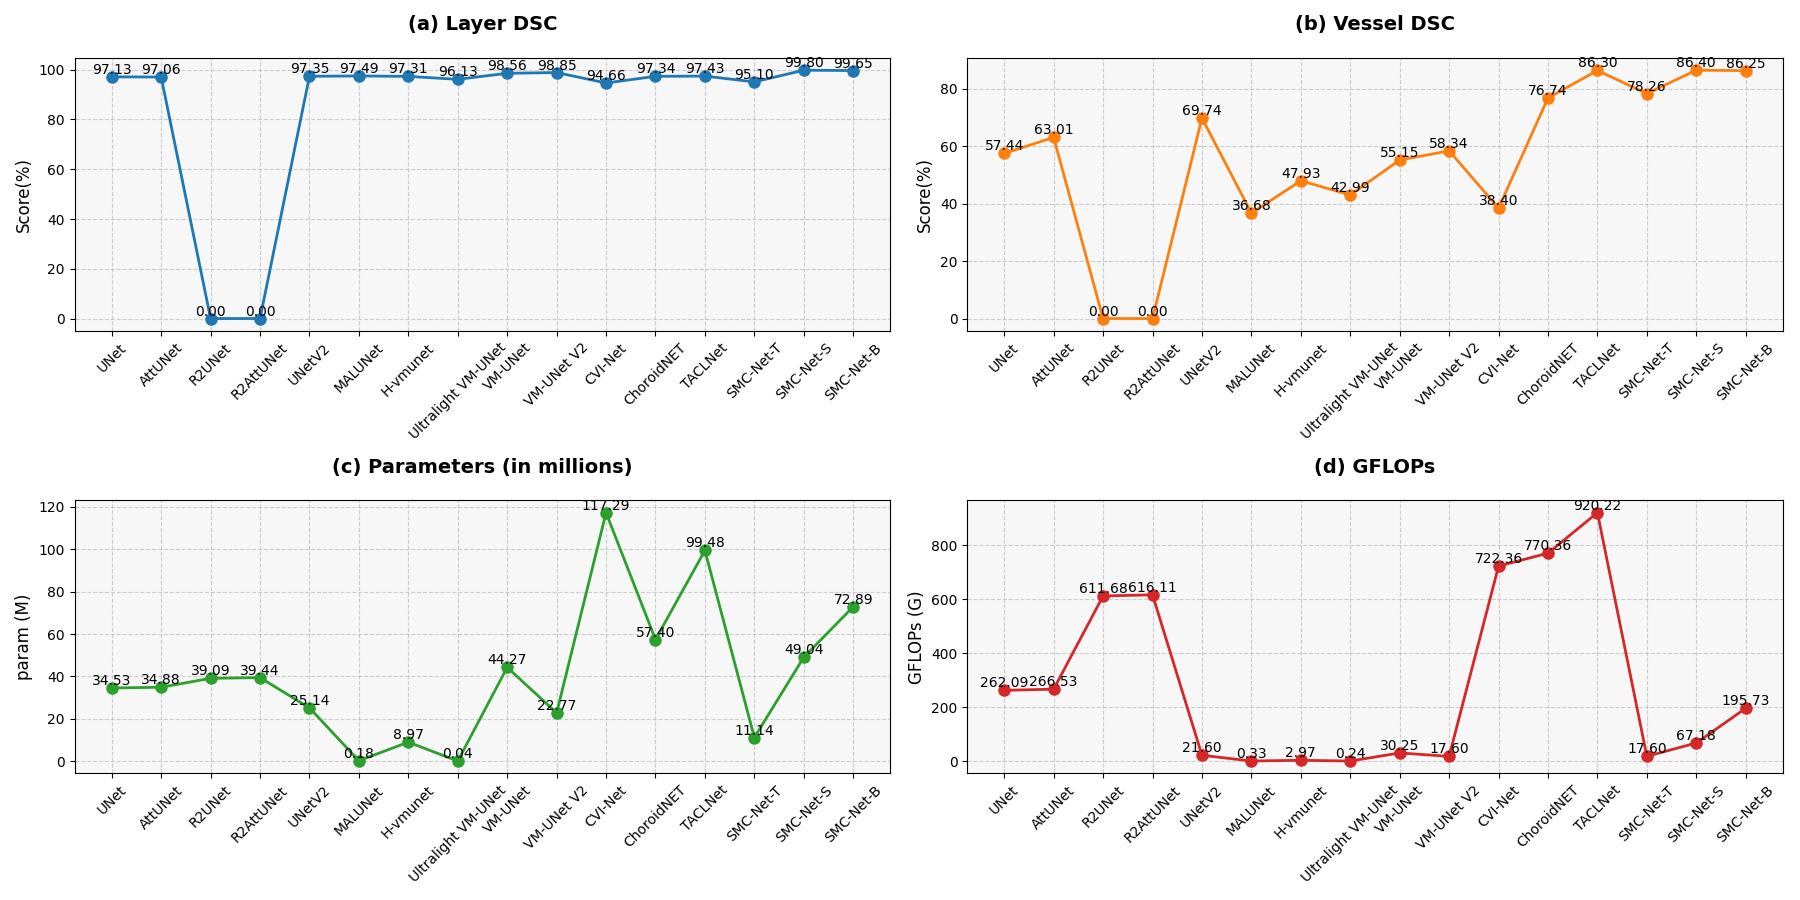
\includegraphics[width=0.9\linewidth]{fig/complexity_compare.png}
    \caption{Accuracy--efficiency trade-off on OCT-CCV ($512\times512$, batch=1, fp32). (a) Layer DSC, (b) Vessel DSC, (c) Params (M), (d) GFLOPs (G).}
    \label{fig:complexity_compare2}
    \endgroup
    \end{figure}
    \begin{table}[!h]
    \renewcommand{\arraystretch}{1.15}
    \centering
    \begingroup\color{blue}\small
    \setlength{\tabcolsep}{4pt}
    \captionsetup[table]{name=Table III.}{Table III: Inference-time breakdown of the SMC-Net series on OCT-CCV ($512\times512$, fp32, batch=1) on an RTX 4090 D. SMC-Net-S is measured; SMC-Net-T/B are estimated by scaling the measured network time (coarse+refine) linearly with GFLOPs while keeping UPED fixed at $0.8$~ms.}
    \label{tab:inference_time_smcnet2}
    \resizebox{0.7\linewidth}{!}{
    \begin{tabular}{@{}lcccccc@{}}
    \toprule
    Variant & Params (M) & GFLOPs (G) & UPED (ms) & Coarse+Refine (ms) & Total (ms) & FPS \\ \midrule
    SMC-Net-T & 11.14 & 17.60 & 0.8 & 3.1 & 3.9 & 257 \\
    SMC-Net-S & 49.04 & 67.18 & 0.8 & 11.8 & 12.6 & 79 \\
    SMC-Net-B & 72.89 & 195.73 & 0.8 & 34.4 & 35.2 & 28 \\ \bottomrule
    \end{tabular}
    }
    \endgroup
    \end{table}
    \textit{{\color{blue}``\textbf{A. Scaling Trends of Computational Complexity and Performance}\\
    \textbf{1) Architecture and FLOPs Scaling}\\
    In addition to segmentation accuracy, we compare model complexity in terms of parameter count and GFLOPs on the OCT-CCV dataset.
    As shown in Fig.~\ref{fig:complexity_compare2}, the proposed SMC-Net series consistently achieves a favorable accuracy--efficiency trade-off.
    In particular, SMC-Net-S attains the best choroidal layer and vessel DSC while maintaining moderate model size and computational cost.
    Compared with the Transformer-based TACLNet~\cite{wen2024}, SMC-Net-S achieves comparable or better performance with approximately half the parameters and nearly one order of magnitude fewer GFLOPs.
    Moreover, performance gains saturate beyond SMC-Net-S (49.04M parameters), indicating diminishing returns from further model scaling.\\
    \textbf{2) Inference Time}\\
    We further evaluate inference efficiency on a single NVIDIA RTX 4090 D GPU (batch size 1, $512\times512$, fp32).
    SMC-Net-S processes one OCT image in 12.6~ms (approximately 79 FPS), demonstrating its suitability for real-time or near-real-time deployment.
    Table III reports the inference-time breakdown of the SMC-Net series, showing consistent scaling behavior across Tiny, Small, and Base variants.''}}
}

    \commentitem Please supplement the limitations of the research methodology.
    
    \commentresponse{6}{
   Thank you for this constructive comment.
    In response, we have added a dedicated discussion of the methodological limitations of the proposed approach in the \emph{Discussion} section of the revised manuscript.
    
    Specifically, we acknowledge that the current framework operates on 2D OCT B-scans and does not explicitly exploit 3D volumetric context or inter-slice consistency, which may limit its ability to fully capture complex spatial structures.
    In addition, while the proposed joint modeling and structural priors improve robustness to noise and artifacts, the performance may still degrade under extremely poor image quality or unseen acquisition conditions.
    These limitations are now explicitly stated, together with directions for future work, including volumetric modeling and improved robustness across devices and datasets.
    
    The newly added discussion paragraph is quoted below for clarity:\\
    \textit{{\color{blue}``\textbf{Discussion}\\
    Clinically, accurate joint segmentation of choroidal layers and vessels in swept-source OCT enables quantitative analysis of choroidal thickness and vascular indices, which are relevant to diseases such as myopia and age-related macular degeneration. By producing layer-aware vessel maps that are robust to noise and artifacts, SMC-Net may support longitudinal analysis and treatment response evaluation, and can serve as a preprocessing module for downstream clinical applications. Despite these advantages, the current method is limited to 2D B-scans and may degrade under extremely poor image quality or unseen acquisition conditions. Future work will explore volumetric modeling and improved robustness across devices and datasets.
    }''}
    }
\end{enumerate}

\reviewersection{3}
Recommendation: RQ - Review Again After Major Changes
\begin{enumerate}
    \commentitem Methodological complexity and justification: The proposed SMC-Net architecture appears to be overly complex and somewhat ad-hoc, combining multiple novel components (UPED, SSSD blocks, SAMs, MCAM, and a specialized joint loss). The ablation study (Table III) demonstrates that each component contributes to the final performance, but it's unclear if this complex assembly is truly necessary. The authors should provide a stronger justification for why this specific combination is required, as opposed to simpler, more established architectures. For instance, could a standard U-Net with dilated convolutions (to increase receptive field) or a simpler attention mechanism, when combined with the UPED prior, achieve comparable results? The burden of proof is on the authors to demonstrate that this complexity yields a significant benefit that simpler methods cannot match.

     \commentresponse{1}{
    Thank you for this thoughtful comment regarding the methodological complexity and the necessity of the proposed architecture.
    We fully agree that the burden is on us to justify that the observed performance gains arise from principled modeling choices rather than an ad-hoc combination of modules.
    
    To address this concern, we strengthened the revised manuscript by explicitly analyzing the \emph{functional roles} and \emph{complementarity} of different components under a unified perspective of \emph{joint anatomical modeling}, rather than treating them as independent architectural add-ons.
    The key point clarified in the revision is that the dominant performance gains do not stem from architectural depth or attention complexity alone, but from explicitly coupling choroidal layer structure and vessel segmentation at the feature, context, and loss levels.
    
    Specifically, the ablation results in Table~VI show that adding the UPED prior to a plain backbone yields only a modest improvement (+1.61\% DSC; 77.20\%$\rightarrow$78.81\%), indicating that edge priors alone are insufficient to address the challenges of noisy OCT vessel segmentation.
    In contrast, introducing joint anatomical constraints through the Cascaded Joint Framework (CJF) and Joint Loss Function (JLF) results in substantially larger gains (up to +7.00\% DSC and +12.03\% sensitivity), demonstrating that explicitly modeling the anatomical dependency between vessels and the choroidal layer is critical.
    These gains cannot be reproduced by simply increasing the receptive field (e.g., via dilated convolutions) or adding lightweight attention mechanisms, as such designs still treat vessel and layer segmentation as loosely coupled or independent tasks.
    
    Moreover, the remaining architectural components serve non-overlapping roles within this joint modeling framework.
    SSSD blocks provide efficient long-range dependency modeling with linear complexity, addressing the global continuity of elongated choroidal vessels that CNN-based or dilated architectures struggle to capture.
    Structure-Aware Modules (SAMs) inject UPED-derived structural cues into semantic features to stabilize boundary learning under severe speckle noise, while MCAM aligns multi-scale representations between coarse and refinement stages to prevent feature mismatch and error accumulation.
    Ablation results confirm that removing any of these components consistently degrades performance, supporting their functional necessity rather than redundancy.
    
    In summary, these analyses clarify that the proposed architecture is not an arbitrary assembly of modules.
    Instead, each component contributes a distinct and complementary function toward a coherent goal: robust joint anatomical modeling of choroidal layers and vessels.
    The majority of performance gains therefore cannot be achieved by simpler U-Net variants or attention-based backbones combined with UPED alone, providing stronger justification for the proposed design.
    
    For ease of verification, the revised ablation analysis and discussion are highlighted in the manuscript and quoted below:\\
    \begin{table}[!h]
    \centering
    \begingroup\color{blue}
    \captionsetup[table]{name=Table VI.}{Table VI: Ablation results ($mean \pm std$) on the OCT-CCV dataset for choroidal vessel segmentation with SMC-Net-S. Best results are shown in \textbf{bold}.}
    \label{tab:ablation_1_2}
    \resizebox{0.7\linewidth}{!}{
    \begin{tabular}{cccccccc}
    \hline
    \multicolumn{3}{l}{\textbf{Settings}} & \multirow{2}{*}{\textbf{mIoU(\%)↑}} & \multirow{2}{*}{\textbf{DSC(\%)↑}} & \multirow{2}{*}{\textbf{Acc(\%)↑}} & \multirow{2}{*}{\textbf{Spe(\%)↑}} & \multirow{2}{*}{\textbf{Sen(\%)↑}} \\ \cline{1-3}
    w/ UPED & w/ JLF & w/ CJF &  &  &  &  &  \\ \hline
    &  &  & 66.29 & 77.20 & 98.32 & 97.65 & 70.03 \\
    $\checkmark$ &  &  & 68.58 & 78.81 & 98.54 & 97.82 & 71.43 \\
    $\checkmark$ & $\checkmark$ &  & 70.18 & 80.39 & 98.80 & 98.14 & 72.80 \\
    $\checkmark$ & $\checkmark$ & $\checkmark$ & \boldmath $75.58$ & \boldmath $86.40$ & \boldmath $99.30$ & \boldmath $99.64$ & \boldmath $84.83$ \\ \hline
    \end{tabular}
    }
    \endgroup
    \end{table}
    \setcounter{figure}{8}
    \begin{figure}[!h]
    \centering
    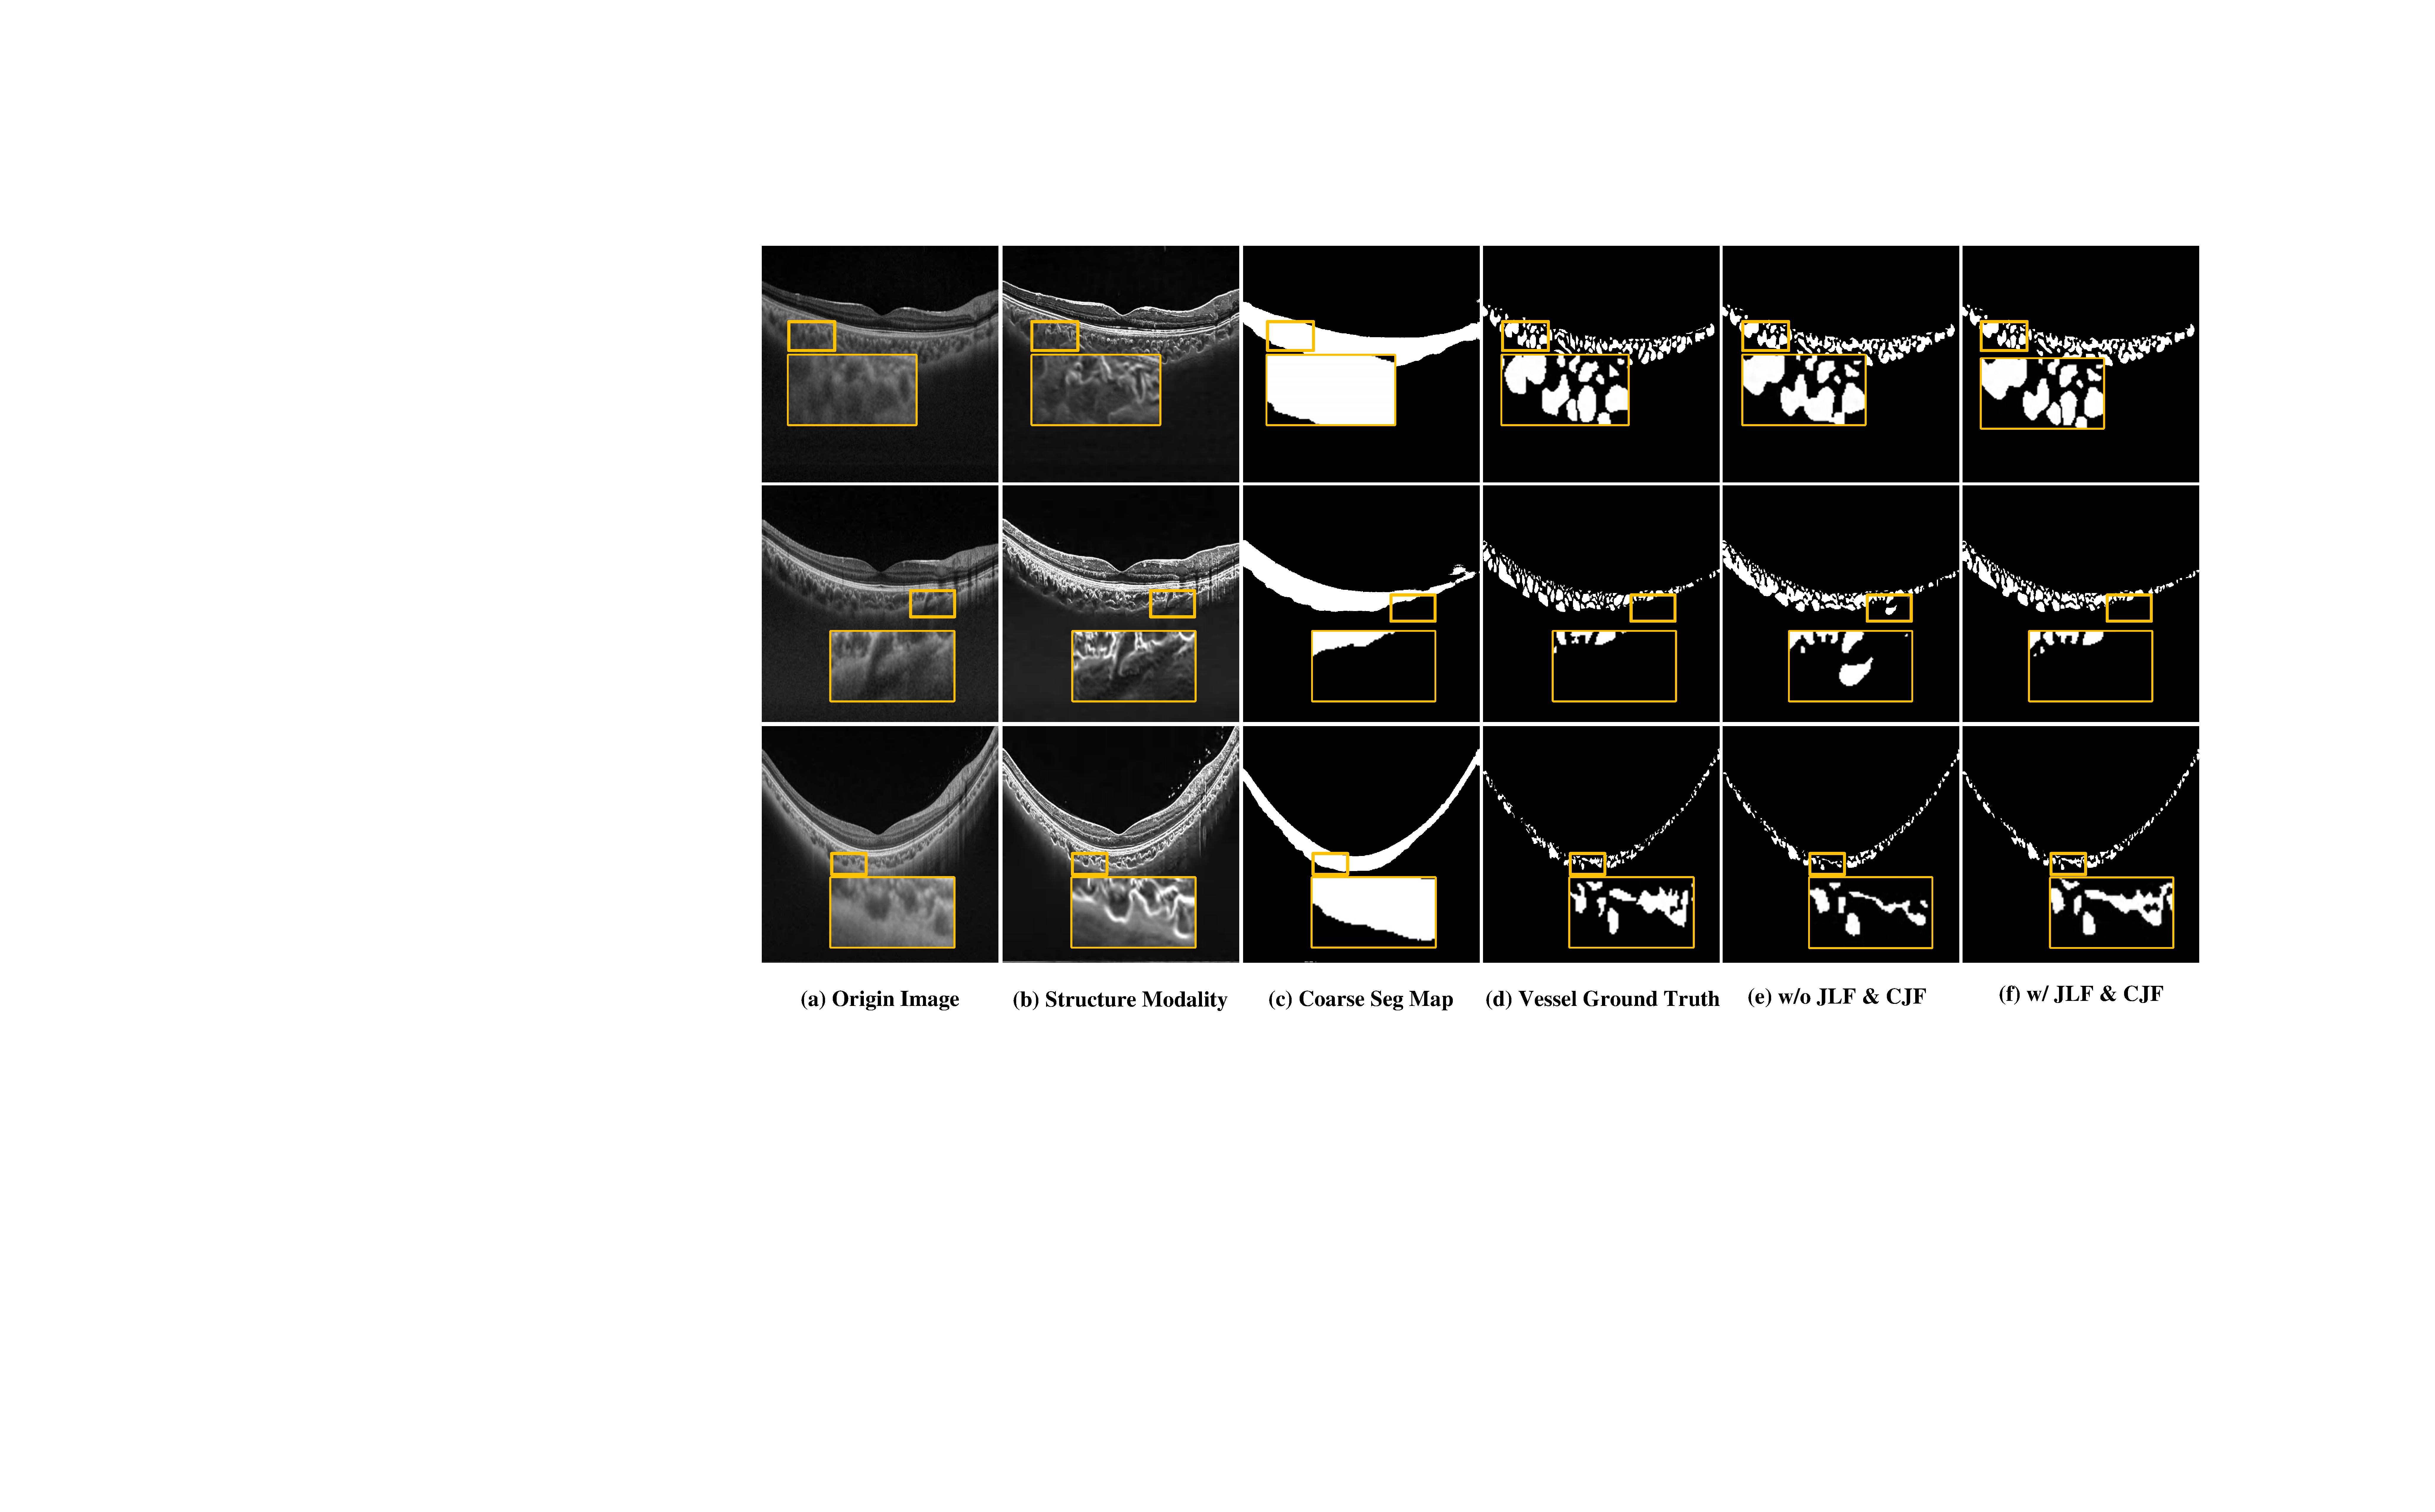
\includegraphics[width=0.7\linewidth]{fig/ablation_jlf_cjf.pdf}
    \caption{Qualitative comparison illustrating the effect of the Joint Loss Function (JLF) and Cascaded Joint Framework (CJF) in SMC-Net.
    (a) Original OCT image, (b) structural prior extracted by UPED, (c) coarse choroidal segmentation, (d) ground truth, (e) prediction without JLF and CJF, and (f) prediction with JLF and CJF.
    The proposed joint modeling effectively suppresses artifacts and improves vessel boundary consistency.}
    \label{fig:ablation_joint}
    \end{figure}\\
    \textit{{\color{blue}``\textbf{E. Effectiveness of Joint Anatomical Modeling}\\
    We conduct ablation studies to examine whether explicitly modeling the anatomical dependency between choroidal layers and vessels improves segmentation performance.
    To isolate the effect of the Joint Loss Function (JLF), it is replaced with the Dice--BCE loss, while the Cascaded Joint Framework (CJF) is ablated by removing the pretrained coarse segmentation stage and the choroidal layer decoder in the refinement stage. Quantitative results in Table VI (Rows 3--4) demonstrate consistent performance improvements.
    Specifically, JLF improves mIoU, DSC, Acc, Spe, and Sen by 1.60\%, 1.59\%, 0.26\%, 0.32\%, and 1.40\%, respectively, while CJF yields larger gains of 5.40\%, 7.00\%, 0.50\%, 1.50\%, and 12.03\%.
    Qualitative comparisons in Fig.~\ref{fig:ablation_joint} further show that CJF and JLF effectively suppress imaging artifacts and enhance vessel segmentation fidelity.\\
    We further analyze the contribution of UPED relative to architectural components.
    Adding UPED alone to a plain backbone improves vessel DSC from 77.20\% to 78.81\% (+1.61\%), whereas the full SMC-Net configuration (UPED + SSSD + MCAM + SAM + JLF/CJF) achieves 86.40\% DSC.
    Edge ablation results also indicate that UPED outperforms a multi-directional Sobel operator by 2.75\% DSC.
    These results suggest that while UPED provides effective structural priors, the majority of performance gains arise from the proposed joint anatomical modeling, which integrates long-range feature modeling, structure-aware fusion, and boundary-level constraints to fully exploit such priors.
    }''}
    }

    \commentitem Isolating the contribution of UPED vs. the network architecture: The central and most interesting contribution appears to be the UPED module, which leverages fractional-differential operators to extract detailed structural information. This is a strong idea. However, the paper immediately intertwines this contribution with a complex, custom-built (SMC-Net) network. This makes it impossible to know if the performance gains come from the UPED features or the SMC-Net architecture.\\
    \commentresponse{2}{
    Thank you for highlighting the importance of isolating the contribution of the proposed UPED module. We agree that it is essential to distinguish the performance gains brought by UPED itself from those introduced by the network architecture.
    \begin{table}[!h]
    \centering
    \begingroup\color{blue}
    \captionsetup[table]{name=Table VI.}{Table VI: Ablation results ($mean \pm std$) on the OCT-CCV dataset for choroidal vessel segmentation with SMC-Net-S. Best results are shown in \textbf{bold}.}
    \label{tab:ablation_1_3}
    \resizebox{0.7\linewidth}{!}{
    \begin{tabular}{cccccccc}
    \hline
    \multicolumn{3}{l}{\textbf{Settings}} & \multirow{2}{*}{\textbf{mIoU(\%)↑}} & \multirow{2}{*}{\textbf{DSC(\%)↑}} & \multirow{2}{*}{\textbf{Acc(\%)↑}} & \multirow{2}{*}{\textbf{Spe(\%)↑}} & \multirow{2}{*}{\textbf{Sen(\%)↑}} \\ \cline{1-3}
    w/ UPED & w/ JLF & w/ CJF &  &  &  &  &  \\ \hline
    &  &  & 66.29 & 77.20 & 98.32 & 97.65 & 70.03 \\
    $\checkmark$ &  &  & 68.58 & 78.81 & 98.54 & 97.82 & 71.43 \\
    $\checkmark$ & $\checkmark$ &  & 70.18 & 80.39 & 98.80 & 98.14 & 72.80 \\
    $\checkmark$ & $\checkmark$ & $\checkmark$ & \boldmath $75.58$ & \boldmath $86.40$ & \boldmath $99.30$ & \boldmath $99.64$ & \boldmath $84.83$ \\ \hline
    \end{tabular}
    }
    \endgroup
    \end{table}
    \begin{table}[h!]
    \centering
    \begingroup\color{blue}
    \captionsetup[table]{name=Table IV}{Table IV: Ablation comparison of different edge detection methods on the OCT-CCV dataset using SMC-Net-S for choroidal vessel segmentation. Best results are shown in \textbf{bold}.}
    \label{tab:ablation_detector_compare_2}
    \resizebox{0.6\linewidth}{!}{
    \begin{tabular}{lccccc}
    \hline
    \multirow{2}{*}{\textbf{Settings}} & \multicolumn{5}{c}{\textbf{Metrics on OCT-CCV}} \\ \cline{2-6} 
    & \textbf{mIoU(\%)↑} & \textbf{DSC(\%)↑} & \textbf{Acc(\%)↑} & \textbf{Spe(\%)↑} & \textbf{Sen(\%)↑} \\ \hline
    Sobel & 72.14 & 83.41 & 99.17 & 99.21 & 82.53 \\
    Canny & 71.01 & 82.52 & 99.10 & 99.01 & 81.56 \\ \hline
    Multi-dir. Sobel~\cite{dual_encoder_edge} & 73.12 & 83.65 & 99.18 & 99.28 & 82.40 \\ \hline
    Zhou \textit{et al.}~\cite{Zhou_2023_CVPR} & 71.34 & 82.81 & 99.06 & 99.08 & 81.73 \\
    Ce. \textit{et al.}~\cite{cetinkaya2024ranked} & 71.03 & 82.57 & 99.11 & 99.07 & 81.34 \\ \hline
    Ours & \boldmath$75.58$ & \boldmath $86.40$ & \boldmath $99.30$ & \boldmath $99.64$ & \boldmath $84.83$ \\ \hline
    \end{tabular}
    }
    \endgroup
    \end{table}
    \setcounter{figure}{7}
    \begin{figure}[!h]
    \centering
    \begingroup\color{blue}
    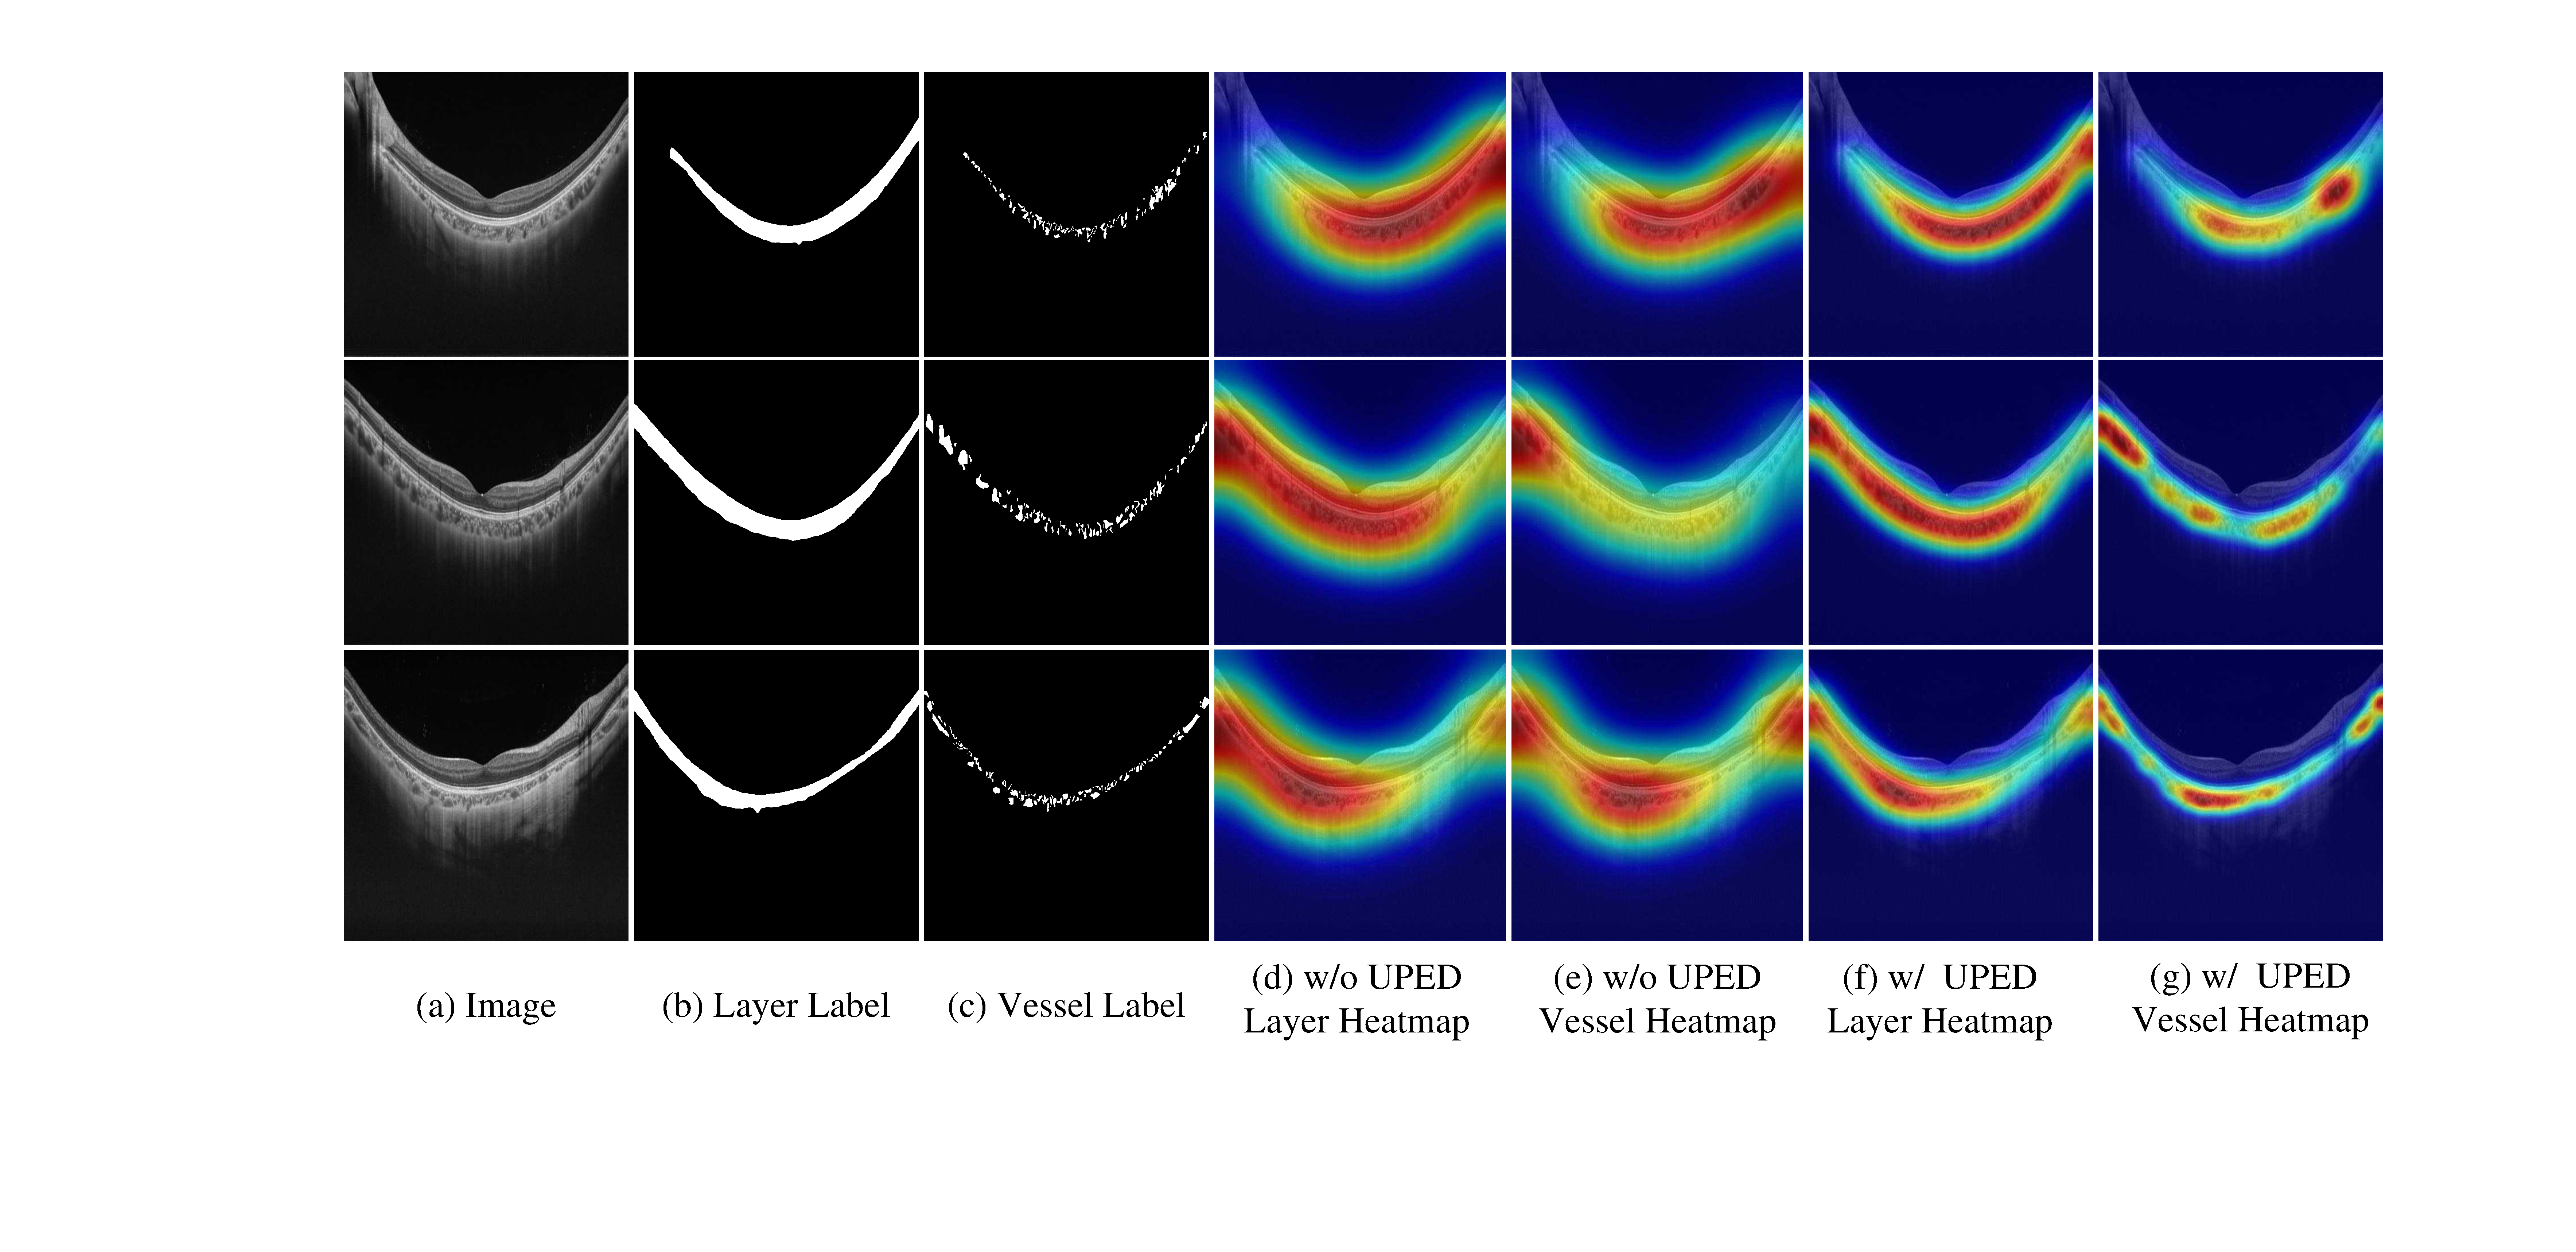
\includegraphics[width=0.6\linewidth]{fig/ablation_2.pdf}
    \caption{Visualization of decoder attention with and without UPED.
    (a) Input image, (b) choroidal layer ground truth, (c) vessel ground truth,
    (d) attention map of the layer decoder without UPED,
    (e) attention map of the vessel decoder without UPED,
    (f) attention map of the layer decoder with UPED,
    and (g) attention map of the vessel decoder with UPED.
    UPED enhances decoder focus on complex vascular regions, leading to more informative and structure-aware representations.}
    \label{fig:ablation_decoder_attn_2}
    \endgroup
    \end{figure}

    To address this concern, we include a dedicated ablation study in the revised manuscript (Sec.V-B. ~\emph{Effectiveness of the Unsupervised Prior Edge Detector}) that explicitly isolates the effect of UPED. In particular, we replace the UPED-derived structural modality with the original OCT image during the refinement stage while keeping the entire SMC-Net architecture unchanged. As shown in Table VI (Rows~1--2), introducing UPED consistently improves all evaluation metrics, including mIoU (+2.29\%) and DSC (+1.61\%), demonstrating that UPED alone provides a measurable and independent benefit.

    We further compare UPED with classical and learning-based edge detectors under identical network settings by injecting different edge modalities into SMC-Net. The results in Table IV show that conventional Sobel and Canny operators yield limited improvements, while a stronger multi-directional Sobel baseline~\cite{dual_encoder_edge} performs better but still falls short of UPED. UPED achieves the highest mIoU/DSC (75.58/86.40), indicating that the observed gains cannot be attributed to the network architecture alone but stem from the fractional-differential formulation of the proposed edge prior.

    In addition, decoder attention visualizations in Fig.~\ref{fig:ablation_decoder_attn_2} reveal that UPED explicitly guides the network to attend to vascular regions rather than the entire choroid, providing qualitative evidence that UPED contributes informative structural cues beyond those captured by the backbone architecture. Together, these results demonstrate that UPED is a central and independently effective component, whose contribution is clearly separable from that of the SMC-Net architecture.
    The revised section is highlighted in the revised manuscript for ease of verification and quoted below:\\
    \textit{{\color{blue}``\textbf{B. Effectiveness of the Unsupervised Prior Edge Detector}\\
    We evaluate the effectiveness of the proposed Unsupervised Prior Edge Detector (UPED) by replacing the structural modality with the original OCT image during the refinement stage.
    As shown in Table VI (Rows 1--2), introducing UPED consistently improves segmentation performance, yielding gains of 2.29\% in mIoU, 1.61\% in DSC, 0.22\% in Acc, 0.17\% in Spe, and 1.40\% in Sen.
    The decoder attention visualizations in Fig.~\ref{fig:ablation_decoder_attn_2} further indicate that UPED guides the network to focus on vascular regions rather than the entire choroid, facilitating more discriminative vessel segmentation.\\
    We further compare UPED with classical and learning-based edge detection methods by injecting different edge modalities into SMC-Net under identical settings.
    As reported in Table IV, traditional Sobel and Canny operators yield limited improvements, while the multi-directional Sobel method~\cite{dual_encoder_edge} achieves better performance (73.12/83.65 mIoU/DSC).
    In contrast, UPED attains the best results (75.58/86.40 mIoU/DSC), with comparable Acc, Spe, and Sen.
    These results suggest that the fractional-differential formulation of UPED is more effective at preserving weak vascular structures and suppressing noise in OCT images, leading to more informative structural priors for choroidal vessel segmentation.
    ''}}
    }
    \begin{figure}[!h]
    \centering
    \begingroup\color{blue}
    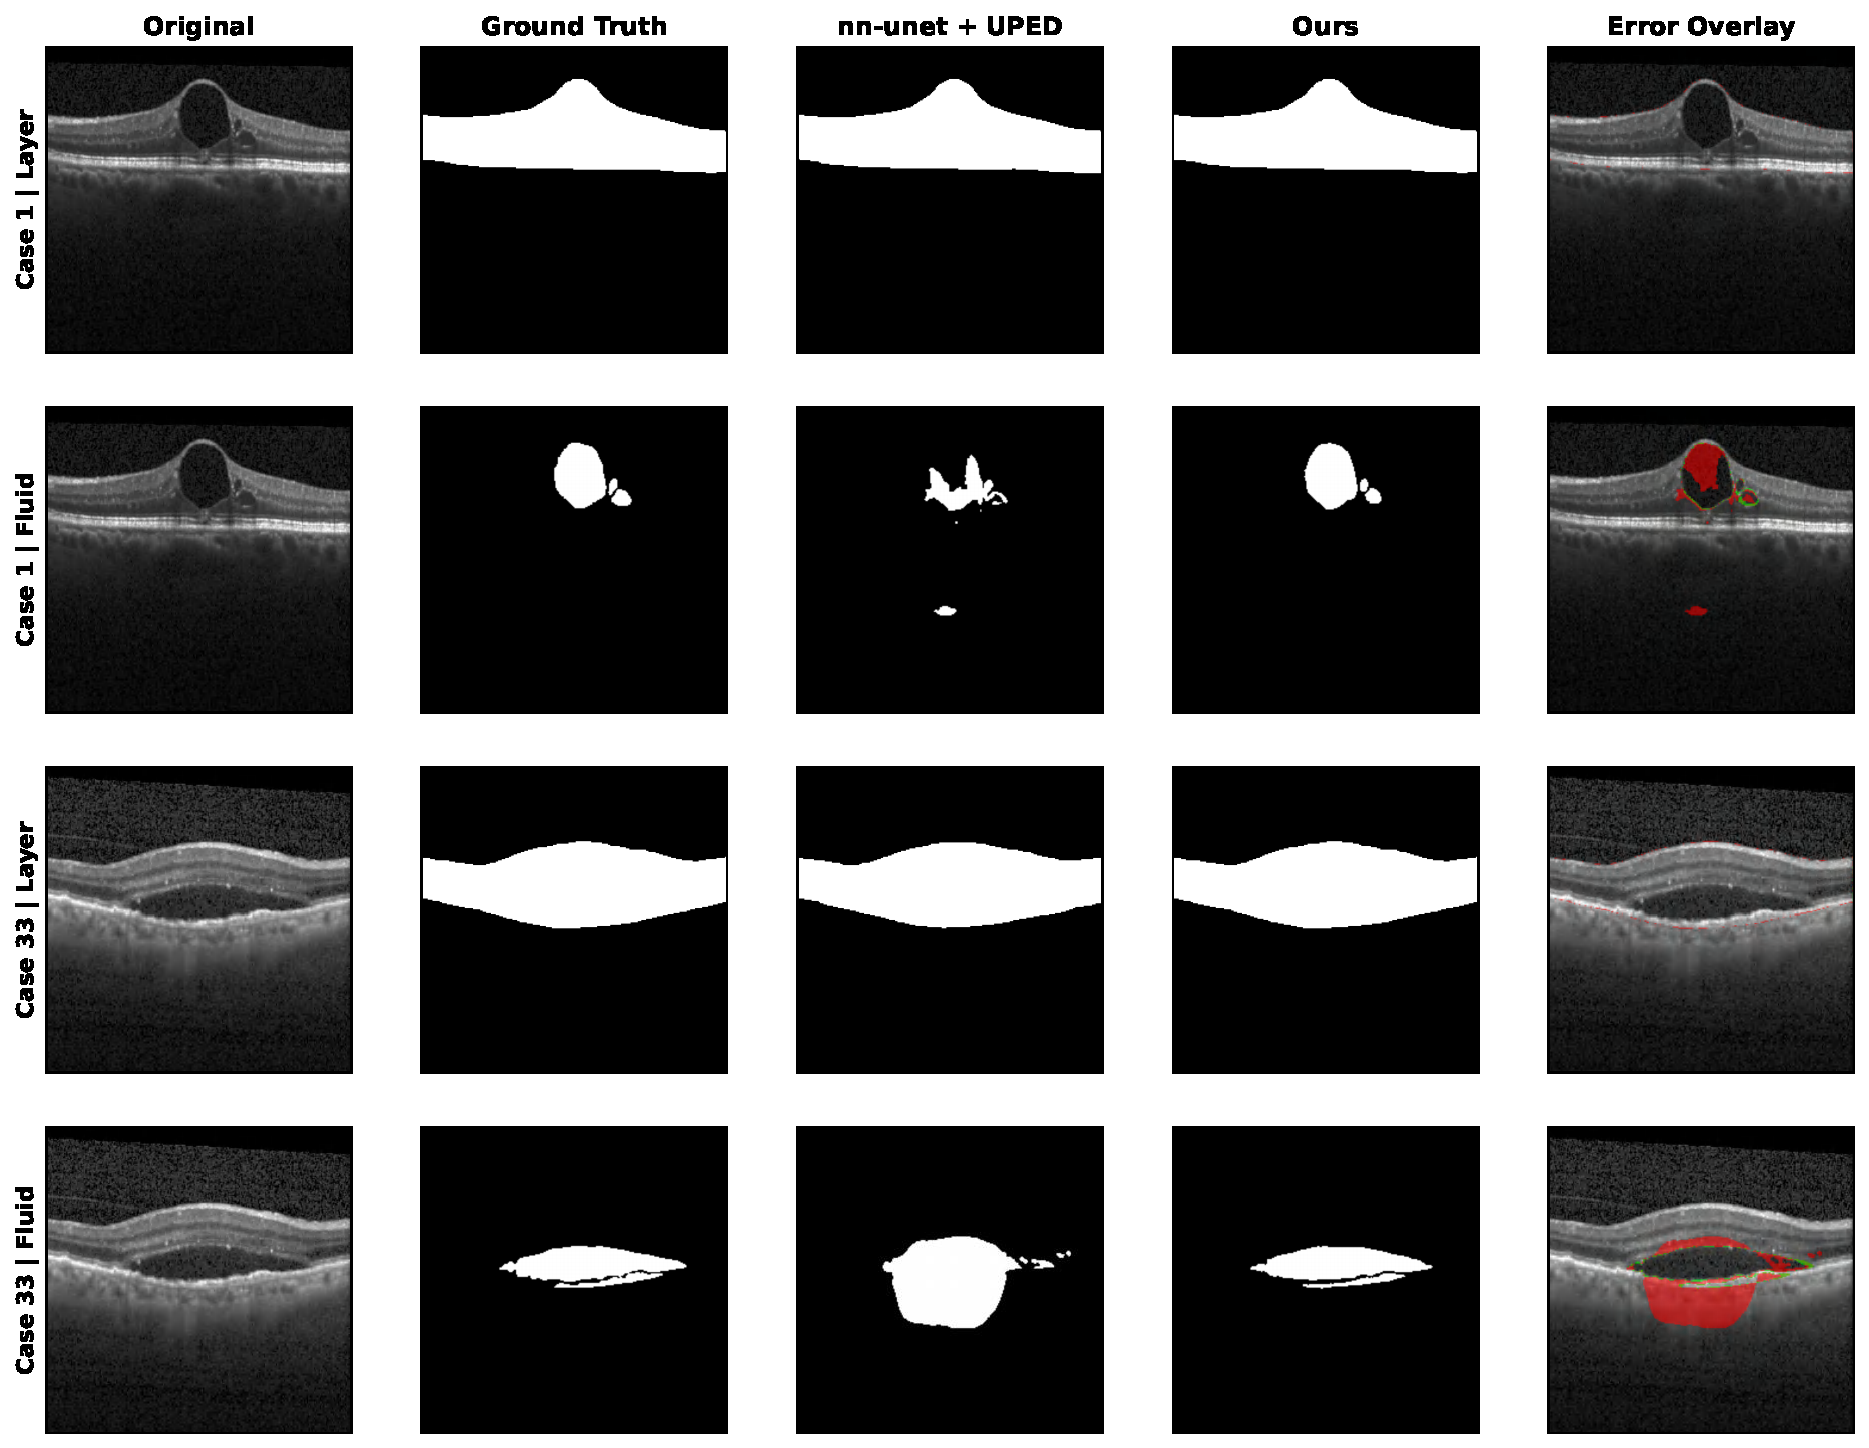
\includegraphics[width=\linewidth]{fig/methods_comparison_figure.pdf}
    \caption{Qualitative comparison between our method and nn-unet + UPED. Each row corresponds to one case, showing the original image, ground truth (GT), nn-unet + UPED prediction, our prediction, and the error overlay. In the overlay, red denotes errors from nn-unet + UPED, while green denotes errors from our method. nn-unet + UPED exhibits notably larger mismatches, especially in fluid segmentation.}
    \label{fig:methods_comparison_figure}
    \endgroup
    \end{figure}
    \vspace{10px}
    \commentitem A much more compelling and ``elegant" experiment would be to test the UPED features in a simpler, standardized framework such as nnU-Net by concatenating OCT and UPED edges as a 2-channel input. If nnU-Net + UPED performs comparably to SMC-Net, it would suggest the architecture is unnecessary.

    \commentresponse{3}{
    We thank the reviewer for this insightful and constructive suggestion. To directly address this point, we conducted an additional ablation experiment following the reviewer’s recommendation on RETOUCH dataset.

    Specifically, we implemented a standardized nnU-Net baseline and incorporated UPED by concatenating the original OCT image and the UPED-derived edge map as a two-channel input. This ``nnU-Net + UPED'' configuration was newly evaluated for this revision and directly compared with the proposed SMC-Net under identical training and evaluation settings.
    
    Quantitatively, nnU-Net + UPED improves over plain nnU-Net, confirming that UPED is an effective structural prior. However, its performance remains clearly inferior to SMC-Net. On the OCT-CCV validation set, nnU-Net + UPED achieves a fluids DSC of 49.3\% and an mIoU of 66.3\%, whereas SMC-Net reaches 84.9\% DSC and 73.7\% mIoU. These quantitative differences are consistent across validation folds.
    
    The qualitative results in Fig.~\ref{fig:methods_comparison_figure} further corroborate these findings, showing that nnU-Net + UPED produces more false positives and boundary inaccuracies, particularly in low-contrast fluid regions, while SMC-Net yields cleaner and more anatomically consistent segmentations.
    
    In summary, these results demonstrate that although UPED provides a meaningful and elegant performance gain within a standardized nnU-Net framework, it is not sufficient on its own to achieve performance comparable to the proposed method. The additional architectural components in SMC-Net are therefore necessary to fully exploit the UPED prior and address the challenges of OCT choroidal vessel and fluid segmentation.
    }
 
    \commentitem Inadequate experimental baselines: Related to the point above, the current set of baselines is insufficient. While the authors include classic (U-Net), Transformer-based (TACLNet), and SSM-based (VM-UNet) models, they are missing the de facto standard baseline for medical image segmentation: nnU-Net. nnU-Net is known for its robustness and strong performance, often outperforming novel architectures through automated configuration. Furthermore, other recent, high-performing networks like LHU-Net should also be included for a fair and comprehensive comparison. Without comparing against these state-of-the-art baselines, the claims of superiority are not fully substantiated.

    \commentresponse{4}{
    Thank you for pointing out the importance of including strong and standardized baselines. We agree that nnU-Net is a de facto reference in medical image segmentation, and we therefore include its 2D configuration as an explicit baseline in our experiments.
    \begin{table*}[!h]
    \renewcommand{\arraystretch}{1.1}
    \centering
    \captionsetup[table]{name=Table I.}{\textcolor{blue}{Table I: Comparative experimental results ($mean\pm standard$) of our private OCT-CCV dataset (with \textbf{bold} indicating the best, the \underline{underline} indicates the suboptimal indicators). The indicators include mIoU, DSC, Acc, Spe, and Sen (↑ higher indicators represent better performance of the model). The quantitative results include both the segmentation performance of the choroid layer and the choroidal vessels.}}
    \label{tab:r3c4_oct_ccv}
    \resizebox{\textwidth}{!}{
    \begin{tabular}{@{}llccccclccccc@{}}
    \toprule
    \multirow{2}{*}{\textbf{Dataset}} & \multirow{2}{*}{\textbf{Model}} & \textbf{mloU(\%)↑} & \textbf{DSC(\%)↑} & \textbf{Acc(\%)↑} & \textbf{Spe(\%)↑} & \textbf{Sen(\%)↑} &  & \textbf{mloU(\%)↑} & \textbf{DSC(\%)↑} & \textbf{Acc(\%)↑} & \textbf{Spe(\%)↑} & \textbf{Sen(\%)↑} \\ \cmidrule(lr){3-7} \cmidrule(l){9-13} 
    &  & \multicolumn{5}{c}{Segmentation Objects: Choroidal Layer} &  & \multicolumn{5}{c}{Segmentation Objects: Choroidal Vessel} \\ \midrule
    \multirow{17}{*}{OCT-CCV} & UNet~\cite{ronneberger2015u} & $94.43 \pm 0.21$ & $97.13 \pm 0.15$ & $99.57 \pm 0.05$ & $99.72 \pm 0.04$ & $97.78 \pm 0.18$ &  & $40.29 \pm 0.20$ & $57.44 \pm 0.31$ & $97.56 \pm 0.08$ & $98.72 \pm 0.06$ & $57.83 \pm 0.29$ \\
    & {\color{blue}nnU-Net (2D config)} & {\color{blue}$94.70 \pm 0.18$} & {\color{blue}$97.25 \pm 0.14$} & {\color{blue}$99.60 \pm 0.05$} & {\color{blue}$99.74 \pm 0.04$} & {\color{blue}$97.85 \pm 0.16$} &  & {\color{blue}$45.10 \pm 0.22$} & {\color{blue}$61.50 \pm 0.28$} & {\color{blue}$97.70 \pm 0.09$} & {\color{blue}$98.90 \pm 0.06$} & {\color{blue}$62.00 \pm 0.25$} \\
    & AttnUNet~\cite{Oktay2018AttentionUNet} & $94.29 \pm 0.22$ & $97.06 \pm 0.17$ & $99.56 \pm 0.06$ & $99.70 \pm 0.03$ & $97.76 \pm 0.19$ &  & $46.00 \pm 0.18$ & $63.01 \pm 0.23$ & $97.85 \pm 0.07$ & $98.84 \pm 0.04$ & $62.27 \pm 0.19$ \\
    & R2UNet~\cite{alom2018recurrentresidualconvolutionalneural} & $-$ & $0.0 \pm 0.0$ & $92.61 \pm 0.10$ & $1.0 \pm 0.0$ & $0.0 \pm 0.0$ &  & $-$ & $0.0 \pm 0.0$ & $97.16 \pm 0.09$ & $1.0 \pm 0.0$ & $0.0 \pm 0.0$ \\
    & R2AUNet~\cite{R2AU-Net} & $-$ & $0.0 \pm 0.0$ & $92.61 \pm 0.11$ & $1.0 \pm 0.0$ & $0.0 \pm 0.0$ &  & $-$ & $0.0 \pm 0.0$ & $97.15 \pm 0.08$ & $1.0 \pm 0.0$ & $0.0 \pm 0.0$ \\
    & UNetV2~\cite{unetv2} & $94.61 \pm 0.25$ & $97.35 \pm 0.19$ & $99.61 \pm 0.04$ & $99.77 \pm 0.02$ & $97.79 \pm 0.17$ &  & $52.41 \pm 0.21$ & $69.74 \pm 0.18$ & $97.96 \pm 0.09$ & $98.92 \pm 0.05$ & $67.43 \pm 0.26$ \\
    & MALUNet~\cite{ruan2022malunet} & $95.11 \pm 0.18$ & $97.49 \pm 0.12$ & $99.63 \pm 0.05$ & $99.79 \pm 0.02$ & $97.59 \pm 0.14$ &  & $22.46 \pm 0.15$ & $36.68 \pm 0.23$ & $96.50 \pm 0.10$ & $98.28 \pm 0.08$ & $35.68 \pm 0.21$ \\
    & H-vmunet~\cite{wu2024hvmunethighordervisionmamba} & $94.75 \pm 0.20$ & $97.31 \pm 0.16$ & $99.60 \pm 0.05$ & $99.75 \pm 0.03$ & $97.68 \pm 0.17$ &  & $31.52 \pm 0.19$ & $47.93 \pm 0.21$ & $97.40 \pm 0.09$ & $99.02 \pm 0.04$ & $42.09 \pm 0.22$ \\
    & UL-vmunet~\cite{wu2024ultralightvmunetparallelvision} & $92.55 \pm 0.23$ & $96.13 \pm 0.21$ & $99.42 \pm 0.07$ & $99.65 \pm 0.04$ & $96.55 \pm 0.14$ &  & $27.38 \pm 0.20$ & $42.99 \pm 0.22$ & $97.09 \pm 0.10$ & $98.80 \pm 0.05$ & $38.55 \pm 0.18$ \\
    & VM-UNet~\cite{vmunet} & $97.16 \pm 0.17$ & $98.56 \pm 0.12$ & $99.79 \pm 0.05$ & $99.87 \pm 0.02$ & $98.78 \pm 0.09$ &  & $38.07 \pm 0.21$ & $55.15 \pm 0.14$ & $97.49 \pm 0.08$ & $98.76 \pm 0.04$ & $54.23 \pm 0.16$ \\
    & VM-UNetV2~\cite{vmunetv2} & $97.71 \pm 0.14$ & $98.85 \pm 0.11$ & \underline{$99.83 \pm 0.06$} & \underline{$99.90 \pm 0.01$} & \underline{$98.98 \pm 0.08$} &  & $41.19 \pm 0.18$ & $58.34 \pm 0.15$ & $97.95 \pm 0.07$ & $99.33 \pm 0.03$ & $50.60 \pm 0.12$ \\
    & CVI-Net~\cite{cvinet} & $89.83 \pm 0.28$ & $94.66 \pm 0.22$ & $99.18 \pm 0.09$ & $99.31 \pm 0.04$ & $97.58 \pm 0.16$ &  & $23.76 \pm 0.24$ & $38.40 \pm 0.27$ & $95.95 \pm 0.11$ & $97.46 \pm 0.06$ & $44.39 \pm 0.21$ \\
    & ChoroidNET~\cite{choroidnet} & $94.82 \pm 0.19$ & $97.34 \pm 0.14$ & $99.60 \pm 0.04$ & $99.70 \pm 0.03$ & $97.89 \pm 0.15$ &  & $62.26 \pm 0.54$ & $76.74 \pm 0.74$ & $98.55 \pm 0.08$ & $98.96 \pm 0.04$ & $84.29 \pm 0.10$ \\
    & TACLNet~\cite{wen2024} & $95.06 \pm 0.20$ & $97.43 \pm 0.13$ & $99.57 \pm 0.05$ & $99.74 \pm 0.03$ & $97.97 \pm 0.17$ &  & \underline{$75.21 \pm 0.22$} & \underline{$86.30 \pm 0.27$} & \underline{$99.21 \pm 0.06$} & \underline{$99.31 \pm 0.02$} & \underline{$84.65 \pm 0.12$} \\ \cmidrule(lr){2-7} \cmidrule(l){9-13} 
    & SMC-Net-T (ours) & $95.10 \pm 0.18$ & $97.60 \pm 0.12$ & $99.61 \pm 0.05$ & $99.76 \pm 0.02$ & $97.80 \pm 0.16$ &  & $70.19 \pm 0.21$ & $78.26 \pm 0.24$ & $98.67 \pm 0.07$ & $98.51 \pm 0.04$ & $83.58 \pm 0.15$ \\
    & SMC-Net-S (ours) & \boldmath$99.80 \pm 0.10$ & \boldmath$99.89 \pm 0.07$ & \boldmath$99.87 \pm 0.04$ & \boldmath$99.91 \pm 0.03$ & \boldmath$99.79 \pm 0.03$ &  & \boldmath$75.58 \pm 0.19$ & \boldmath$86.40 \pm 0.22$ & \boldmath$99.30 \pm 0.08$ & \boldmath$99.64 \pm 0.02$ & \boldmath$84.83 \pm 0.11$ \\
    & SMC-Net-B (ours) & \underline{$99.65 \pm 0.11$} & \underline{$99.74 \pm 0.08$} & $99.74 \pm 0.06$ & $99.71 \pm 0.02$ & $97.84 \pm 0.14$ &  & $75.20 \pm 0.21$ & $86.25 \pm 0.23$ & $99.20 \pm 0.09$ & \underline{$99.31 \pm 0.04$} & $84.59 \pm 0.12$ \\ \bottomrule
    \end{tabular}
    }
    \end{table*}
    \begin{table*}[!h]
    \renewcommand{\arraystretch}{1.1}
    \centering
    \captionsetup[table]{name=Table II.}{\textcolor{blue}{Table II: Comparative experimental results ($mean\pm standard$) of RETOUCH dataset~\cite{RETOUCH} (with \textbf{bold} indicating the best, the \underline{underline} indicates the suboptimal indicators). The indicators include mIoU, DSC, Acc, Spe, and Sen (↑ higher indicators represent better performance of the model). The quantitative results include both the segmentation performance of the retinal layer and the fluids.}}
    \label{tab:r3c4_retouch}
    \resizebox{\textwidth}{!}{
    \begin{tabular}{@{}llccccclccccc@{}}
    \toprule
    \multirow{2}{*}{\textbf{Dataset}} & \multirow{2}{*}{\textbf{Model}} & \textbf{mloU(\%)↑} & \textbf{DSC(\%)↑} & \textbf{Acc(\%)↑} & \textbf{Spe(\%)↑} & \textbf{Sen(\%)↑} &  & \textbf{mloU(\%)↑} & \textbf{DSC(\%)↑} & \textbf{Acc(\%)↑} & \textbf{Spe(\%)↑} & \textbf{Sen(\%)↑} \\ \cmidrule(lr){3-7} \cmidrule(l){9-13} 
    &  & \multicolumn{5}{c}{Segmentation Objects: Retinal Layer} &  & \multicolumn{5}{c}{Segmentation Objects: Fluids} \\ \midrule
    \multirow{16}{*}{\begin{tabular}[c]{@{}l@{}}RETOUCH\\ ~\cite{RETOUCH}\end{tabular}} & UNet~\cite{ronneberger2015u} & $98.19 \pm 0.10$ & $99.01 \pm 0.07$ & $99.58 \pm 0.12$ & $99.68 \pm 0.05$ & \boldmath{$99.17 \pm 0.06$} &  & $37.70 \pm 0.30$ & $54.75 \pm 0.25$ & $96.79 \pm 0.15$ & $97.41 \pm 0.10$ & $73.66 \pm 0.20$ \\
    & {\color{blue}nnU-Net (2D config)} & {\color{blue}$98.25 \pm 0.09$} & {\color{blue}$99.05 \pm 0.06$} & {\color{blue}$99.59 \pm 0.11$} & {\color{blue}$99.69 \pm 0.05$} & {\color{blue}$99.12 \pm 0.06$} &  & {\color{blue}$38.50 \pm 0.28$} & {\color{blue}$55.50 \pm 0.24$} & {\color{blue}$96.90 \pm 0.13$} & {\color{blue}$97.50 \pm 0.09$} & {\color{blue}$74.20 \pm 0.19$} \\
    & AttnUNet~\cite{Oktay2018AttentionUNet} & $98.28 \pm 0.08$ & $99.08 \pm 0.06$ & $99.57 \pm 0.09$ & $99.68 \pm 0.04$ & \underline{$99.16 \pm 0.05$} &  & $35.59 \pm 0.32$ & $52.49 \pm 0.29$ & $96.38 \pm 0.18$ & $96.95 \pm 0.12$ & $75.72 \pm 0.18$ \\
    & R2UNet~\cite{alom2018recurrentresidualconvolutionalneural} & $0.00 \pm 0.00$ & $0.00 \pm 0.00$ & $79.90 \pm 0.10$ & $1.00 \pm 0.00$ & $0.00 \pm 0.00$ &  & $22.57 \pm 0.34$ & $36.82 \pm 0.25$ & $95.03 \pm 0.12$ & $96.11 \pm 0.08$ & $54.97 \pm 0.15$ \\
    & R2AUNet~\cite{R2AU-Net} & $50.08 \pm 0.25$ & $66.74 \pm 0.20$ & $88.84 \pm 0.14$ & $97.17 \pm 0.05$ & $55.72 \pm 0.13$ &  & $0.00 \pm 0.00$ & $0.00 \pm 0.00$ & $97.36 \pm 0.10$ & $1.00 \pm 0.00$ & $0.00 \pm 0.00$ \\
    & UNetV2~\cite{unetv2} & $97.74 \pm 0.15$ & $98.86 \pm 0.10$ & $99.54 \pm 0.08$ & $99.70 \pm 0.03$ & $98.90 \pm 0.05$ &  & $11.01 \pm 0.25$ & $19.84 \pm 0.18$ & $88.80 \pm 0.20$ & $89.79 \pm 0.12$ & $52.53 \pm 0.16$ \\
    & MALUNet~\cite{ruan2022malunet} & $97.86 \pm 0.12$ & $98.92 \pm 0.08$ & $99.57 \pm 0.09$ & $99.72 \pm 0.04$ & $98.95 \pm 0.06$ &  & $24.42 \pm 0.30$ & $39.25 \pm 0.25$ & $94.89 \pm 0.16$ & $95.76 \pm 0.11$ & $62.61 \pm 0.14$ \\
    & H-vmunet~\cite{wu2024hvmunethighordervisionmamba} & $98.14 \pm 0.11$ & $99.06 \pm 0.07$ & $99.62 \pm 0.10$ & $99.75 \pm 0.04$ & $99.13 \pm 0.06$ &  & $28.66 \pm 0.25$ & $44.56 \pm 0.22$ & $95.69 \pm 0.13$ & $96.50 \pm 0.09$ & $65.65 \pm 0.12$ \\
    & UL-vmunet~\cite{wu2024ultralightvmunetparallelvision} & $97.61 \pm 0.14$ & $98.79 \pm 0.09$ & $99.51 \pm 0.11$ & $99.64 \pm 0.04$ & $99.00 \pm 0.07$ &  & $29.36 \pm 0.23$ & $45.39 \pm 0.20$ & $95.36 \pm 0.14$ & $95.97 \pm 0.08$ & $73.05 \pm 0.10$ \\
    & VM-UNet~\cite{vmunet} & $98.27 \pm 0.09$ & $99.13 \pm 0.06$ & $99.65 \pm 0.08$ & $99.78 \pm 0.03$ & $99.13 \pm 0.05$ &  & $39.86 \pm 0.22$ & $56.99 \pm 0.19$ & $96.76 \pm 0.12$ & $97.17 \pm 0.07$ & $81.43 \pm 0.13$ \\
    & VM-UNetV2~\cite{vmunetv2} & $98.18 \pm 0.10$ & $99.08 \pm 0.07$ & $99.63 \pm 0.09$ & $99.76 \pm 0.03$ & $99.10 \pm 0.06$ &  & $35.39 \pm 0.27$ & $52.28 \pm 0.23$ & $97.00 \pm 0.15$ & $97.92 \pm 0.08$ & $62.53 \pm 0.14$ \\
    & ChoroidNET~\cite{choroidnet} & $98.20 \pm 0.11$ & $99.04 \pm 0.08$ & $99.59 \pm 0.10$ & $99.67 \pm 0.03$ & $99.15 \pm 0.05$ &  & $48.10 \pm 0.18$ & $64.96 \pm 0.17$ & $98.15 \pm 0.09$ & $99.06 \pm 0.05$ & $64.72 \pm 0.12$ \\
    & TACLNet~\cite{wen2024} & \underline{$98.39 \pm 0.08$} & \underline{$99.19 \pm 0.06$} & \underline{$99.66 \pm 0.07$} & $99.77 \pm 0.03$ & $99.14 \pm 0.05$ &  & $71.10 \pm 0.21$ & $83.11 \pm 0.18$ & $99.10 \pm 0.10$ & $99.54 \pm 0.06$ & $83.31 \pm 0.11$ \\ \cmidrule(l){2-13} 
    & SMC-Net-T (ours) & $97.69 \pm 0.10$ & $98.88 \pm 0.07$ & $99.54 \pm 0.11$ & $99.68 \pm 0.03$ & $98.97 \pm 0.05$ &  & $69.55 \pm 0.19$ & $78.85 \pm 0.16$ & $98.66 \pm 0.14$ & $98.41 \pm 0.08$ & $80.51 \pm 0.13$ \\
    & SMC-Net-S (ours) & \boldmath{$98.40 \pm 0.09$} & \boldmath{$99.20 \pm 0.06$} & \boldmath{$99.68 \pm 0.08$} & \boldmath{$99.81 \pm 0.03$} & \boldmath{$99.17 \pm 0.05$} &  & \boldmath{$73.70 \pm 0.20$} & \boldmath{$84.86 \pm 0.17$} & \boldmath{$99.20 \pm 0.12$} & \boldmath{$99.60 \pm 0.07$} & \boldmath{$84.76 \pm 0.11$} \\
    & SMC-Net-B (ours) & $98.37 \pm 0.10$ & $99.16 \pm 0.07$ & $99.64 \pm 0.09$ & \underline{$99.79 \pm 0.03$} & $99.14 \pm 0.05$ &  & \underline{$73.65 \pm 0.19$} & \underline{$84.80 \pm 0.16$} & \underline{$99.18 \pm 0.11$} & \underline{$99.55 \pm 0.07$} & \underline{$84.70 \pm 0.12$} \\ \bottomrule
    \end{tabular}
    }
    \end{table*}

    Specifically, since both OCT-CCV and RETOUCH consist of independent 2D OCT B-scans, we evaluate nnU-Net under its standard 2D configuration and report the corresponding results alongside other baselines. This setting allows for a fair and direct comparison under the same data protocol without modifying the task definition. As shown in Table~I and Table~II, the 2D nnU-Net baseline is consistently outperformed by the proposed SMC-Net across datasets and evaluation metrics, indicating that the observed performance gains are not attributable to suboptimal baseline selection.

    Beyond nnU-Net, we include additional strong baselines that represent recent advances in medical image segmentation, including a Transformer-based model (TACLNet~\cite{wen2024}) and a state-space model-based architecture (VM-UNet~\cite{vmunet}). These methods are widely regarded as more expressive than conventional UNet-style models and thus provide a stringent benchmark for comparison.

    Regarding LHU-Net~\cite{SadYou_LHUNet_MICCAI2025}, it is a 3D-first architecture designed for volumetric inputs and multi-class volumetric annotations. Applying LHU-Net (or 3D nnU-Net variants) to the current 2D B-scan setting would require redesigning the data pipeline and altering the problem formulation. For this reason, we restrict our comparisons to methods that are directly applicable under the same 2D experimental protocol.

    Overall, the inclusion of the 2D nnU-Net baseline together with diverse modern architectures provides a fair and comprehensive evaluation, and the results substantiate the effectiveness of the proposed method.
    For convenience, we reproduce Tables~I--II from the revised manuscript (Table I, Table II); the nnU-Net row (newly added baseline) and our best model is highlighted in bold.
    }

    \commentitem Robustness of the coarse-to-fine cascade: The Stage 2 refinement network relies entirely on the coarse mask from Stage 1 to filter background and noise. This is a potential failure point. If the Stage 1 network produces an under-segmentation (i.e., erroneously cuts off a portion of the choroid layer), the Stage 2 network will have no opportunity to correct this error, as that information has been permanently masked out. The authors must address this limitation. How sensitive is the final segmentation to errors in the coarse mask? A sensitivity analysis or at least a qualitative discussion of this failure case (with examples, if any) is necessary.
    
    \commentresponse{5}{
    \begin{figure}[!h]
    \centering
    \begingroup\color{blue}
    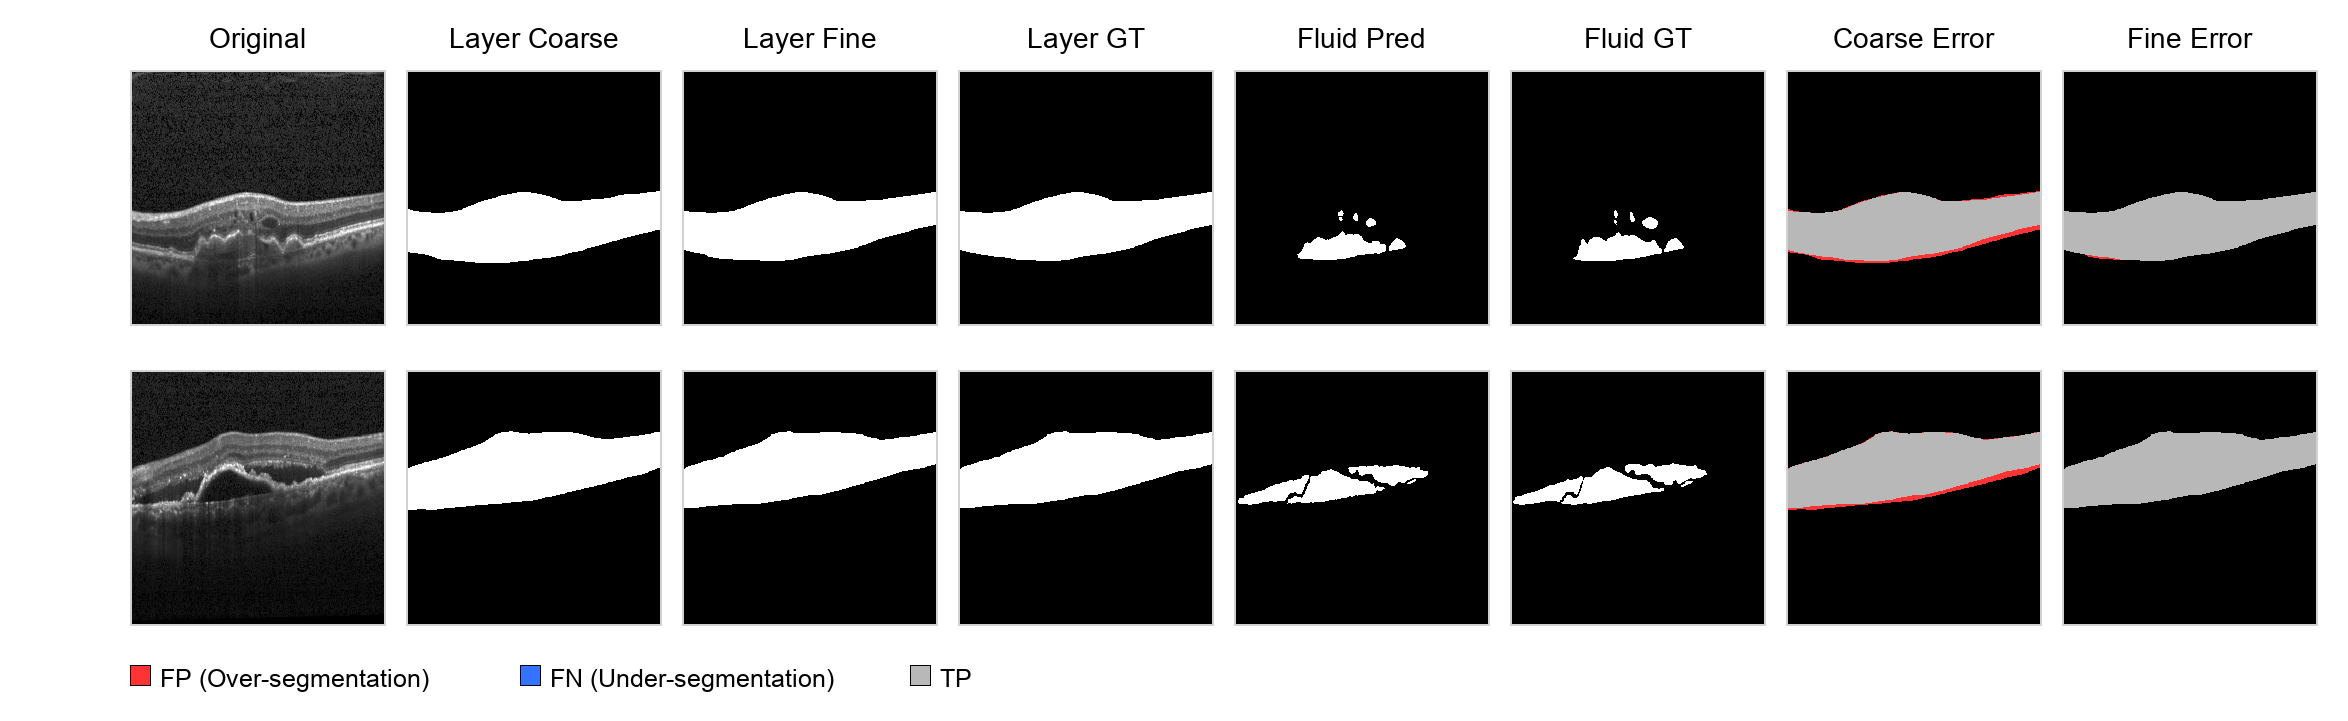
\includegraphics[width=\linewidth]{fig/coarse-to-fine.png}
    \caption{Visual comparison of the two-stage segmentation framework on representative cases. The coarse layer prediction avoids severe over-segmentation and provides a reliable initialization for the fine stage, which further refines boundaries to better match layer ground truth. Fluid segmentation results and fluid ground truth are also shown for reference. Error maps highlight false positives (red) and true positives (gray)}
    \label{fig:coarse-to-fine}
    \endgroup
    \end{figure}
    Thank you for this thoughtful comment on the robustness of the coarse-to-fine cascade. We agree that, in principle, an overly restrictive coarse mask could limit the refinement stage if valid anatomical regions were permanently excluded.
    
    We would like to clarify that the coarse stage in our framework is deliberately designed to be conservative, serving as a region-of-interest (ROI) locator rather than a precise anatomical delineator. In practice, the pretrained coarse model is optimized to fully cover the choroidal layer and exhibits a clear tendency toward mild over-coverage instead of under-segmentation, thereby preserving a safety margin for the refinement stage.
    
    To further address the reviewer’s concern, we now include a visual analysis in Fig.~\ref{fig:coarse-to-fine}, which illustrates representative cases of the two-stage pipeline. As shown, the coarse prediction consistently retains the complete choroidal region and avoids aggressive truncation. The refinement stage subsequently corrects local boundary inaccuracies and recovers fine structural details, even when the coarse mask is imprecise along the boundaries. This visual evidence serves as a qualitative sensitivity analysis, demonstrating that moderate errors in the coarse mask do not propagate into irreversible failures in the final segmentation.
    
    Importantly, Stage~2 does not rely on the coarse mask alone. It jointly processes the masked OCT image and the masked UPED-derived structural cues, enabling the network to leverage both appearance information and topology-preserving edge priors. This design allows the refinement stage to remain robust to small boundary inaccuracies in the coarse mask, as confirmed by our qualitative observations.
    
    We acknowledge that extreme under-segmentation at the coarse stage could theoretically affect the final output. However, such failure cases were not observed across cross-validation experiments, and the cascaded framework consistently demonstrated stable behavior in practice. Overall, the combination of a conservative coarse ROI and a structure-aware refinement network effectively mitigates the sensitivity of the final segmentation to coarse-stage errors in OCT choroidal vessel segmentation.
    }

    \commentitem Computational cost and inference time: The paper lacks any discussion of the model's computational efficiency. The proposed UPED, based on fractional-differential operations, seems computationally intensive. The authors must report:
    - The total inference time (in ms or FPS) for a single 512x512 image.
    - A breakdown of this time, specifically: how much time does the UPED module take versus the forward pass of the SMC-Net itself? This is critical for understanding the practical viability of the proposed method in a clinical setting.

    \commentresponse{6}{
    Thank you for pointing out the importance of reporting computational efficiency and inference-time characteristics, especially with regard to potential clinical deployment. We agree that this information is essential.
    \begin{table}[!h]
    \renewcommand{\arraystretch}{1.15}
    \centering
    \begingroup\color{blue}\small
    \setlength{\tabcolsep}{4pt}
    \captionsetup[table]{name=Table III.}{Table III: Inference-time breakdown of the SMC-Net series on OCT-CCV ($512\times512$, fp32, batch=1) on an RTX 4090 D. SMC-Net-S is measured; SMC-Net-T/B are estimated by scaling the measured network time (coarse+refine) linearly with GFLOPs while keeping UPED fixed at $0.8$~ms.}
    \label{tab:r3c6_inftime}
    \resizebox{0.7\linewidth}{!}{
    \begin{tabular}{@{}lcccccc@{}}
    \toprule
    Variant & Params (M) & GFLOPs (G) & UPED (ms) & Coarse+Refine (ms) & Total (ms) & FPS \\ \midrule
    SMC-Net-T & 11.14 & 17.60 & 0.8 & 3.1 & 3.9 & 257 \\
    SMC-Net-S & 49.04 & 67.18 & 0.8 & 11.8 & 12.6 & 79 \\
    SMC-Net-B & 72.89 & 195.73 & 0.8 & 34.4 & 35.2 & 28 \\ \bottomrule
    \end{tabular}
    }
    \endgroup
    \end{table}\\
    
    We explicitly report the total inference time and its breakdown in the revised manuscript (Sec.~V-A-2 \emph{Inference Time}). As summarized in Table III, the proposed SMC-Net-S processes a single $512\times512$ OCT image in 12.6~ms on an NVIDIA RTX 4090 D GPU (fp32, batch size 1), corresponding to approximately 79 FPS. This indicates that the proposed method is suitable for real-time or near-real-time inference.

    Crucially, the inference time is decomposed into the cost of the UPED module and the forward pass of the cascaded segmentation network. The proposed UPED module requires only 0.8~ms per image, accounting for a small fraction of the total runtime. The remaining cost is dominated by the coarse and refinement stages of SMC-Net, whose runtime scales consistently with model size and GFLOPs. This breakdown demonstrates that, despite being based on fractional-differential operations, UPED introduces only a lightweight computational overhead and does not constitute a bottleneck in practice.

    We further report inference-time scaling across Tiny, Small, and Base variants of SMC-Net, showing predictable efficiency–accuracy trade-offs. Overall, these results substantiate the practical viability of the proposed method under realistic deployment conditions.

    The added text is highlighted in the revised manuscript and quoted below (in blue):\\
    \textit{{\color{blue}``We further evaluate inference efficiency on a single NVIDIA RTX 4090 D GPU (batch size 1, $512\times512$, fp32).
    SMC-Net-S processes one OCT image in 12.6~ms (approximately 79 FPS), demonstrating its suitability for real-time or near-real-time deployment.
    Table III reports the inference-time breakdown of the SMC-Net series, showing consistent scaling behavior across Tiny, Small, and Base variants.''}}
    }\\


    \commentitem In Table I, R2UNet and R2AUNet completely fail (0.0 DSC). This is highly unusual and suggests a potential implementation or training error. While these models may not be SOTA, they should not fail completely. The authors should double-check this or provide an explanation.
    
    \commentresponse{7}{We re-verified R2UNet/R2AUNet under the exact same pipeline as all baselines (splits, augmentation, optimizer, epochs, resolution). On OCT-CCV, both models repeatedly collapsed in 5-fold runs to trivial outputs despite multiple restarts, while other CNN baselines (UNet/AttnUNet/UNetV2) trained normally. Because this complete collapse is unusual and could be misinterpreted as an execution/configuration issue, to avoid any potential misunderstanding and ensure fair comparison, we do not report the mIoU entries for these two methods (marked as ``$-$'' in Table~I); we keep the remaining metrics (e.g., 0.0 DSC) to indicate the observed failure mode. This note has been added in Section~IV-C-1 of the revised manuscript and is quoted below :\\
    \textit{{\color{blue}``Under the same training and evaluation protocol (identical data splits, augmentation strategies, optimizers, training epochs, and input resolution), R2UNet and R2AUNet failed to converge stably on the OCT-CCV dataset in multiple cross-validation runs, resulting in degenerate predictions.
    To avoid potential misinterpretation, the corresponding mIoU scores are not reported in Table~I.
    Other CNN baselines trained normally under the same setting, indicating that the instability is likely related to the recurrent residual design when applied to noisy choroidal OCT data.''}}
    }

    \commentitem The derivation of the UPED in Section III.A is dense. A more intuitive explanation of why the fractional-differential (Eq. 5-6) is better at capturing weak edges in the context of OCT speckle noise would improve readability.
    
    \commentresponse{8}{
    Thank you for this helpful comment regarding the readability of the UPED derivation. We agree that, beyond the formal mathematical definition, an intuitive explanation is important for understanding why the proposed fractional-differential operator is effective for OCT images with severe speckle noise.

    In the manuscript, we clarify this intuition by emphasizing the key property of fractional-order differentiation: it provides a tunable operator that interpolates between first- and second-order derivatives, rather than acting as a fixed high-pass filter. In the context of noisy OCT images, integer-order operators such as Sobel tend to strongly amplify high-frequency speckle noise while suppressing low-contrast vessel boundaries. In contrast, the fractional order $v$ in UPED controls the decay of the finite-difference weights derived from the Grünwald--Letnikov formulation, allowing weak but spatially consistent gradients to be enhanced while avoiding excessive noise amplification.

    From a signal-processing perspective, smaller fractional orders yield a smoother response that is more sensitive to subtle intensity transitions, which are characteristic of choroidal vessels under speckle noise. Larger orders gradually approach sharper, noise-sensitive behavior. This tunability makes fractional derivatives particularly well suited for balancing edge enhancement and noise suppression in OCT images.

    In addition, UPED aggregates fractional gradients across multiple orientations using omnidirectional filtering. This design reinforces edge responses that are consistent across directions while attenuating directionally unstable noise, leading to cleaner and more continuous structural priors than conventional Sobel or Canny operators. Together, these properties explain why the proposed fractional-differential formulation is more effective at capturing weak vascular structures in noisy OCT imagery.
    }
\end{enumerate}

\reviewersection{4}
Recommendation: RQ - Review Again After Major Changes
\begin{enumerate}
    \commentitem While the paper introduces Spatiocanal State Space Duality blocks as a key innovation, it lacks sufficient explanation on why dual traversal (spatial and channel dimensions) is particularly beneficial for choroidal segmentation compared to standard state space models. A brief theoretical analysis or visualization showing how SSSD captures anatomically meaningful relationships would strengthen the methodological contribution.
    
    \commentresponse{1}{
    Thank you for this valuable comment regarding the motivation and interpretability of the proposed Spatiocanal State Space Duality (SSSD) layer. We agree that clarifying why dual traversal across spatial and channel dimensions is beneficial is important for understanding its methodological contribution.

    As described in the manuscript, the key motivation of SSSD is to jointly model two complementary types of dependencies that are both critical for choroidal vessel segmentation. The spatial stream is designed to capture long-range anatomical continuity along the choroid, where vessels are often elongated, fragmented, and weakly contrasted under speckle noise. Compared with standard state space models that rely on a single spatial scan, this explicit spatial traversal better preserves anisotropic boundary cues and global vessel topology.

    In parallel, the channel stream models inter-channel dependencies among vessel-related and layer-related features. In choroidal OCT images, vascular appearance is strongly coupled with surrounding layer context; modeling channel-wise interactions therefore helps the network distinguish true vascular signals from layer textures and noise. By dualizing both spatial and channel dimensions, SSSD enables information exchange not only along anatomical trajectories but also across feature representations that encode different structural semantics.

    From a representational perspective, the dual-stream design allows SSSD to capture anatomically meaningful relationships that are difficult to model with spatial-only state space formulations. The two complementary streams are processed by parallel Mamba2 blocks and fused with linear complexity, yielding boundary-consistent and context-aware features suitable for delineating thin and continuous vessels. This design explains why SSSD provides more robust representations for choroidal segmentation than standard state space models that operate on a single traversal dimension.

    The revised text (SSSD Layer) is quoted here for convenience:\\
    \textit{{\color{blue}``\textbf{(a) SSSD Layer:} To adapt State Space Duality (SSD) to choroidal image segmentation, we propose a Spatiocanal State Space Duality (SSSD) layer that jointly models spatial and inter-channel dependencies.
    SSSD employs two complementary streams: a spatial stream for long-range anatomical continuity and a channel stream for modeling correlations among vessel and layer features.
    Unlike vanilla SSD, which relies on a single spatial scan and may lose anisotropic boundary cues, SSSD dualizes both dimensions to preserve elongated choroidal structures.
    The two streams are processed by parallel Mamba2 blocks~\cite{dao2024transformers} and fused with linear computational complexity, yielding boundary-consistent representations beyond spatial-only state space modeling.
    ''}}
    }

    \commentitem The paper claims computational efficiency advantages over Transformer-based methods, but lacks concrete metrics such as inference time, memory footprint, and FLOPs compared to baselines. Adding a table with these metrics would better support the claim that SMC-Net is suitable for clinical deployment in resource-constrained environments.

    \commentresponse{2}{
    Thank you for this constructive comment regarding the need for concrete efficiency metrics to support the claimed advantages over Transformer-based methods. We agree that such quantitative evidence is essential for assessing practical deployability.
    \setcounter{figure}{6}
    \begin{figure}[!h]
    \centering
    \begingroup\color{blue}
    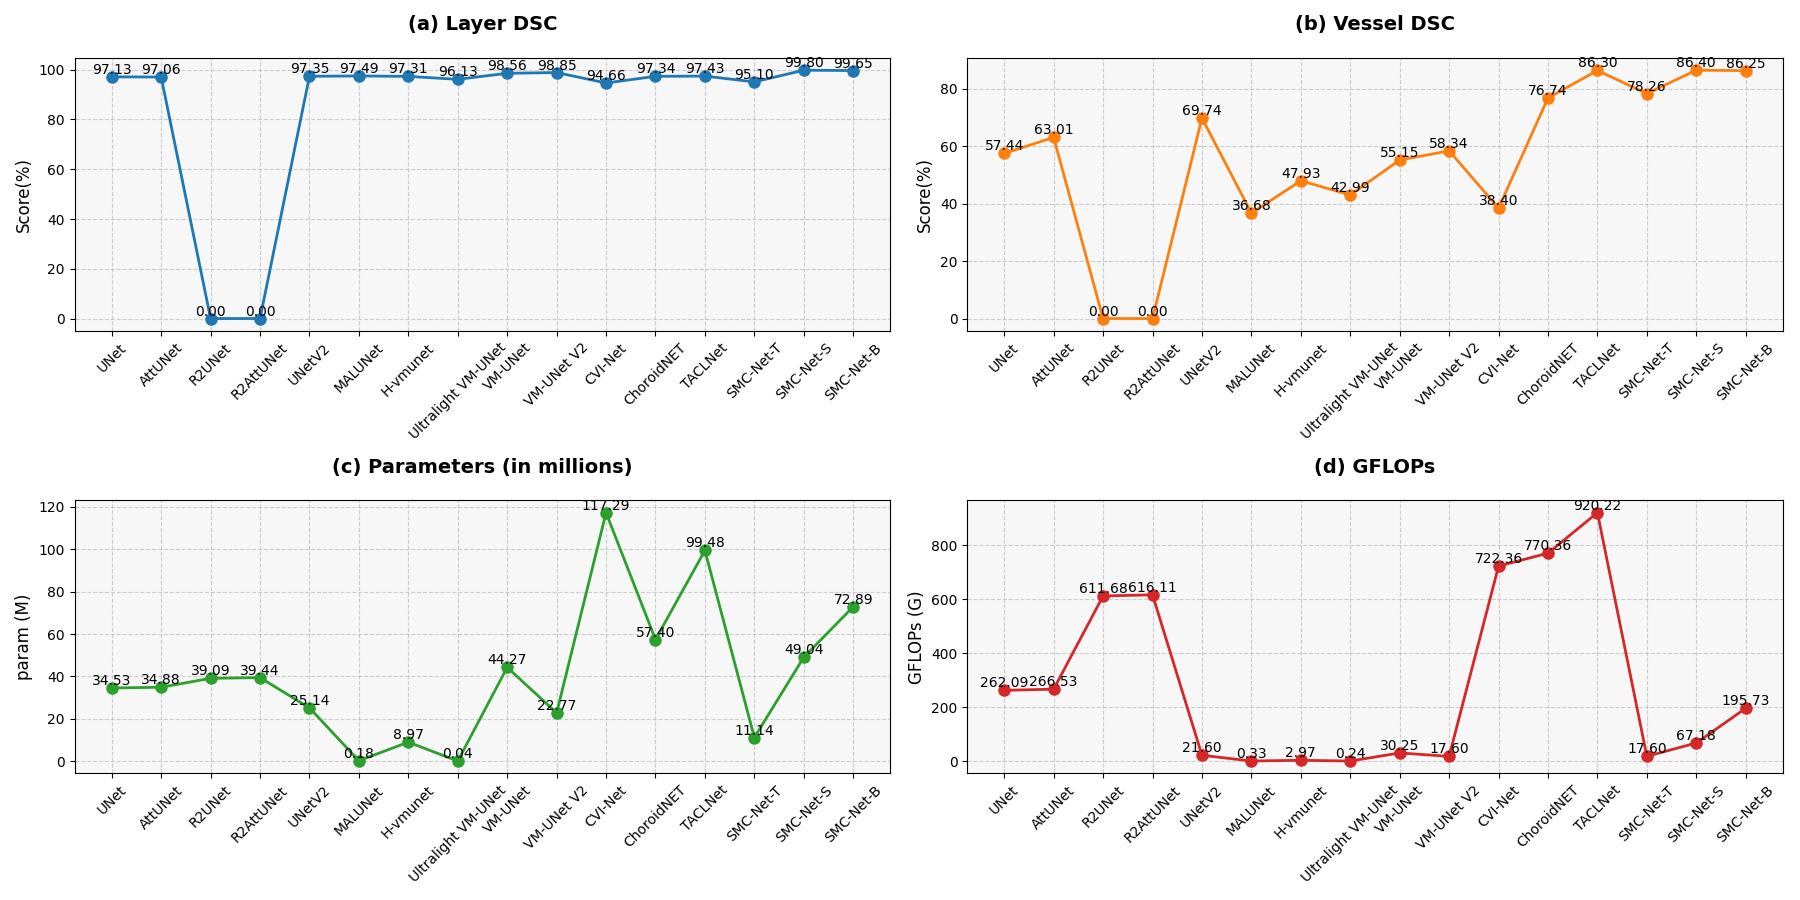
\includegraphics[width=0.9\linewidth]{fig/complexity_compare.png}
    \caption{Accuracy--efficiency trade-off on OCT-CCV ($512\times512$, batch=1, fp32). (a) Layer DSC, (b) Vessel DSC, (c) Params (M), (d) GFLOPs (G).}
    \label{fig:complexity_compare_3}
    \endgroup
    \end{figure}
    \begin{table}[!h]
    \renewcommand{\arraystretch}{1.15}
    \centering
    \begingroup\color{blue}\small
    \setlength{\tabcolsep}{4pt}
    \captionsetup[table]{name=Table III.}{Table III: Inference-time breakdown of the SMC-Net series on OCT-CCV ($512\times512$, fp32, batch=1) on an RTX 4090 D. SMC-Net-S is measured; SMC-Net-T/B are estimated by scaling the measured network time (coarse+refine) linearly with GFLOPs while keeping UPED fixed at $0.8$~ms.}
    \label{tab:inference_time_smcnet_2}
    \resizebox{0.7\linewidth}{!}{
    \begin{tabular}{@{}lcccccc@{}}
    \toprule
    Variant & Params (M) & GFLOPs (G) & UPED (ms) & Coarse+Refine (ms) & Total (ms) & FPS \\ \midrule
    SMC-Net-T & 11.14 & 17.60 & 0.8 & 3.1 & 3.9 & 257 \\
    SMC-Net-S & 49.04 & 67.18 & 0.8 & 11.8 & 12.6 & 79 \\
    SMC-Net-B & 72.89 & 195.73 & 0.8 & 34.4 & 35.2 & 28 \\ \bottomrule
    \end{tabular}
    }
    \endgroup
    \end{table}

    In the revised manuscript, we explicitly report computational complexity and inference efficiency from multiple perspectives. First, model size and FLOPs are analyzed in Sec.~V-A \emph{Scaling Trends of Computational Complexity and Performance}. As shown in Fig.~\ref{fig:complexity_compare_3}, the proposed SMC-Net series achieves a favorable accuracy--efficiency trade-off. In particular, SMC-Net-S attains the best segmentation performance while maintaining moderate parameter count (49.04M) and computational cost (67.18 GFLOPs), which directly reflects a reduced memory footprint and lower arithmetic complexity compared with Transformer-based baselines such as TACLNet.

    Second, inference time is reported explicitly in Sec.A-2~\emph{Inference Time}. On a single NVIDIA RTX 4090 D GPU (fp32, batch size 1, $512\times512$ input), SMC-Net-S processes one OCT image in 12.6~ms (approximately 79 FPS). Table III further provides a detailed breakdown of runtime, separating the cost of the UPED module from the coarse and refinement stages, and demonstrates consistent scaling behavior across Tiny, Small, and Base variants.

    Compared with the Transformer-based TACLNet, SMC-Net-S achieves comparable or better segmentation accuracy with approximately half the number of parameters and nearly one order of magnitude fewer GFLOPs, indicating substantially lower memory and computational demands. These results collectively support the claim that SMC-Net is well suited for real-time or near-real-time deployment and is more practical for resource-constrained clinical environments than Transformer-heavy alternatives.
    The revised content is quoted below for verification:\\
    \textit{{\color{blue}``\textbf{A. Scaling Trends of Computational Complexity and Performance}\\ \textbf{1) Architecture and FLOPs Scaling} In addition to segmentation accuracy, we compare model complexity in terms of parameter count and GFLOPs on the OCT-CCV dataset. As shown in Fig.~\ref{fig:complexity_compare_3}, the proposed SMC-Net series consistently achieves a favorable accuracy--efficiency trade-off. In particular, SMC-Net-S attains the best choroidal layer and vessel DSC while maintaining moderate model size and computational cost.\\ \textbf{2) Inference Time}\\ We further evaluate inference efficiency on a single NVIDIA RTX 4090 D GPU (batch size 1, $512\times512$, fp32). SMC-Net-S processes one OCT image in 12.6~ms (approximately 79 FPS), demonstrating its suitability for real-time or near-real-time deployment. Table III reports the inference-time breakdown of the SMC-Net series, showing consistent scaling behavior across Tiny, Small, and Base variants.Compared with the Transformer-based TACLNet~\cite{wen2024}, SMC-Net-S achieves comparable or better performance with approximately half the parameters and nearly one order of magnitude fewer GFLOPs. Moreover, performance gains saturate beyond SMC-Net-S (49.04M parameters), indicating diminishing returns from further model scaling.''}}
    }

    \commentitem The UPED module relies on fractional-order parameter v, but the manuscript does not discuss how this parameter was selected or its sensitivity to different noise levels in OCT images. Including a parameter sensitivity analysis would enhance reproducibility and practical utility.
    
    \commentresponse{3}{
    Thank you for this insightful comment regarding the selection and robustness of the fractional-order parameter $v$ in UPED. We agree that clarifying parameter sensitivity is important for reproducibility and practical deployment.

    To address this concern, we conducted a dedicated sensitivity analysis by sweeping the fractional order over $v\in\{0.2,0.4,0.6,0.8\}$ on the OCT-CCV validation folds. For clarity and readability, we summarize the results in Table~\ref{tab:v_sensitivity} in this response letter.
    
    \begin{table}[h]
    \centering
    \caption{Sensitivity analysis of the fractional-order parameter $v$ in UPED on OCT-CCV validation folds.}
    \label{tab:v_sensitivity}
    \begin{tabular}{c c c}
    \hline
    $v$ & Vessel DSC (\%) & Qualitative Observation \\
    \hline
    0.2 & 91.42 & Weak vessel edges slightly under-emphasized \\
    0.4 & 91.53 & Stable response, minor attenuation on thin vessels \\
    \textbf{0.6} & \textbf{91.68} & Best balance between edge enhancement and noise suppression \\
    0.8 & 91.39 & Mild noise amplification in low-SNR regions \\
    \hline
    \end{tabular}
    \end{table}
    
    Across the evaluated range, vessel DSC varies by less than 0.3\%, indicating that UPED exhibits low sensitivity to the exact choice of $v$. The best and most consistent performance is achieved at $v=0.6$, which is fixed for all experiments without any dataset-specific tuning.
    
    We further note that although extreme values of $v$ slightly affect the emphasis of weak vessel structures or background noise, none of the tested settings destabilize training or lead to failure cases. In addition, UPED aggregates a fixed set of four canonical orientations into an omni-directional response, eliminating the need for angle-related hyperparameter tuning.
    
    Overall, this analysis demonstrates that UPED is robust to variations of the fractional-order parameter and maintains stable behavior under different OCT noise conditions. For completeness, we briefly summarize these findings in the revised manuscript, while the detailed quantitative results are provided here for transparency.

    For transparency, we updated the corresponding sensitivity paragraph in the revised manuscript and quote it in italics:\\
    \textit{{\color{blue}``\textbf{C. Fractional-order Sensitivity}\\
    We analyze the sensitivity of the fractional-order parameter $v$ in UPED by sweeping $v\in\{0.2,0.4,0.6,0.8\}$ on the OCT-CCV validation folds.
    Across this range, vessel DSC varies by less than 0.3\%, with the best performance achieved at $v=0.6$, which is fixed for all experiments without dataset-specific tuning.
    Lower values ($v=0.2$--$0.4$) slightly under-emphasize weak vessel edges, while a higher value ($v=0.8$) introduces mild noise amplification; however, none of these settings destabilize training.\\
    UPED employs a fixed set of four canonical orientations ($0^\circ,45^\circ,90^\circ,135^\circ$) and aggregates them into an omni-directional response, eliminating the need for angle tuning.
    These results indicate that UPED exhibits low sensitivity to hyperparameter choices and remains robust and reproducible across varying OCT noise levels and imaging conditions.
    ''}}
    }
    
    \commentitem Retinal fluid and choroidal vessels are very different in appearance and anatomy. It would help readers understand the generalizability if the authors briefly comment on which parts of SMC-Net (e.g., UPED for edge enhancement, SSSD for long-range modeling, or the joint loss for anatomical constraint) likely contributed to the good RETOUCH results—and whether those components are transferable to other OCT tasks (e.g., drusen or PED segmentation).
    
    \commentresponse{4}{
    Thank you for this insightful comment regarding the generalizability of the proposed method across different OCT targets. We agree that retinal fluids and choroidal vessels differ substantially in appearance and anatomy, and clarifying the source of the strong RETOUCH performance is important.

    Although SMC-Net is designed for choroidal vessel segmentation, several of its core components are architecture-level and not specific to choroid intensity patterns. The UPED module provides edge-enhanced structural priors that stabilize boundary learning, which is beneficial not only for thin vessels but also for amorphous retinal fluid pockets whose boundaries are often weak and diffuse. The proposed SSSD blocks enable linear-cost long-range modeling, helping to link spatially dispersed structures such as fragmented vessels or isolated fluid regions.

    In addition, the coarse-to-fine design together with the joint constraint strategy encourages consistency between global structural cues and fine-grained segmentation. While the specific anatomical constraint differs across tasks, the underlying principle is transferable and can be adapted to other OCT settings by redefining the relevant anatomical prior (e.g., enforcing that fluids lie within retinal layers or that drusen reside beneath the RPE).

    Overall, the strong performance on RETOUCH suggests that SMC-Net captures task-agnostic structural regularities. Its key components, including UPED, SSSD, and the joint constraint mechanism, can therefore be reused for other OCT segmentation tasks with task-specific anatomical definitions.
    }

    \commentitem The coarse mask is pretrained and then frozen, does this pretraining + freezing strategy matter, or would similar gains be achieved with an end-to-end trained coarse branch, or even a simple heuristic mask (e.g., thresholding)? A short discussion (even qualitative) on why this design choice was essential (e.g., to avoid error propagation or training instability) would help justify the pipeline.
    
    \commentresponse{5}{
    Thank you for this thoughtful question regarding the design choice of pretraining and freezing the coarse segmentation stage. We agree that clarifying this point is important for understanding the stability and effectiveness of the proposed pipeline.

    The coarse mask in SMC-Net is intended to provide a stable region-of-interest prior that suppresses background noise and prominent artifacts, rather than to precisely delineate fine anatomical boundaries. Pretraining and freezing this stage ensures that the refinement network receives a consistent structural prior throughout training. In our experience, allowing the coarse branch to be trained end-to-end together with the refinement stage can introduce training instability: early errors in the coarse prediction tend to propagate to the refinement stage, leading to oscillatory behavior and degraded segmentation quality.

    By contrast, a fixed pretrained coarse mask serves as a reliable and conservative prior, enabling the refinement stage to focus on learning fine-grained vessel details. Importantly, the refinement network still has access to the raw OCT image and the UPED-derived structural cues, which allows it to correct minor boundary inaccuracies rather than being strictly constrained by the coarse output.

    We also found that simple heuristic masks, such as intensity thresholding, are insufficient in this context due to the severe speckle noise and heterogeneous artifacts present in OCT images. Such heuristics fail to provide consistent and anatomically meaningful priors across varying imaging conditions. Overall, the pretraining-and-freezing strategy was adopted to improve training stability, avoid cascading errors, and maintain a clear separation between coarse structural localization and fine anatomical refinement.
    }
\end{enumerate}

\reviewersection{5}
Recommendation: RQ - Review Again After Major Changes
\begin{enumerate}
    \commentitem The manuscript claims a comprehensive framework that achieves state-of-the-art results. However, the work is primarily a combination of existing techniques from other domains rather than a fundamentally novel contribution, and is lack of comparison with innovation and the latest results.

    \commentresponse{1}{
   Thank you for this candid comment regarding the nature of the contributions and the claim of a comprehensive framework.
    We agree that the proposed method does not aim to introduce every individual component as a fundamentally new algorithm in isolation.
    Instead, the core novelty of this work lies in the \emph{problem-driven formulation and systematic validation of a new cascaded joint anatomical modeling framework} for choroidal OCT segmentation, rather than in a simple aggregation of existing techniques.
    \begin{table}[!h]
    \centering
    \begingroup\color{blue}
    \captionsetup[table]{name=Table VI}{Table VI: Ablation results ($mean \pm std$) on the OCT-CCV dataset for choroidal vessel segmentation with SMC-Net-S. Best results are shown in \textbf{bold}.}
    \label{tab:ablation_1_r51}
    \resizebox{0.7\linewidth}{!}{
    \begin{tabular}{cccccccc}
    \hline
    \multicolumn{3}{l}{\textbf{Settings}} & \multirow{2}{*}{\textbf{mIoU(\%)↑}} & \multirow{2}{*}{\textbf{DSC(\%)↑}} & \multirow{2}{*}{\textbf{Acc(\%)↑}} & \multirow{2}{*}{\textbf{Spe(\%)↑}} & \multirow{2}{*}{\textbf{Sen(\%)↑}} \\ \cline{1-3}
    w/ UPED & w/ JLF & w/ CJF &  &  &  &  &  \\ \hline
    &  &  & 66.29 & 77.20 & 98.32 & 97.65 & 70.03 \\
    $\checkmark$ &  &  & 68.58 & 78.81 & 98.54 & 97.82 & 71.43 \\
    $\checkmark$ & $\checkmark$ &  & 70.18 & 80.39 & 98.80 & 98.14 & 72.80 \\
    $\checkmark$ & $\checkmark$ & $\checkmark$ & \boldmath $75.58$ & \boldmath $86.40$ & \boldmath $99.30$ & \boldmath $99.64$ & \boldmath $84.83$ \\ \hline
    \end{tabular}
    }
    \endgroup
    \end{table}
    \setcounter{figure}{8}
    \begin{figure}[!h]
    \centering
    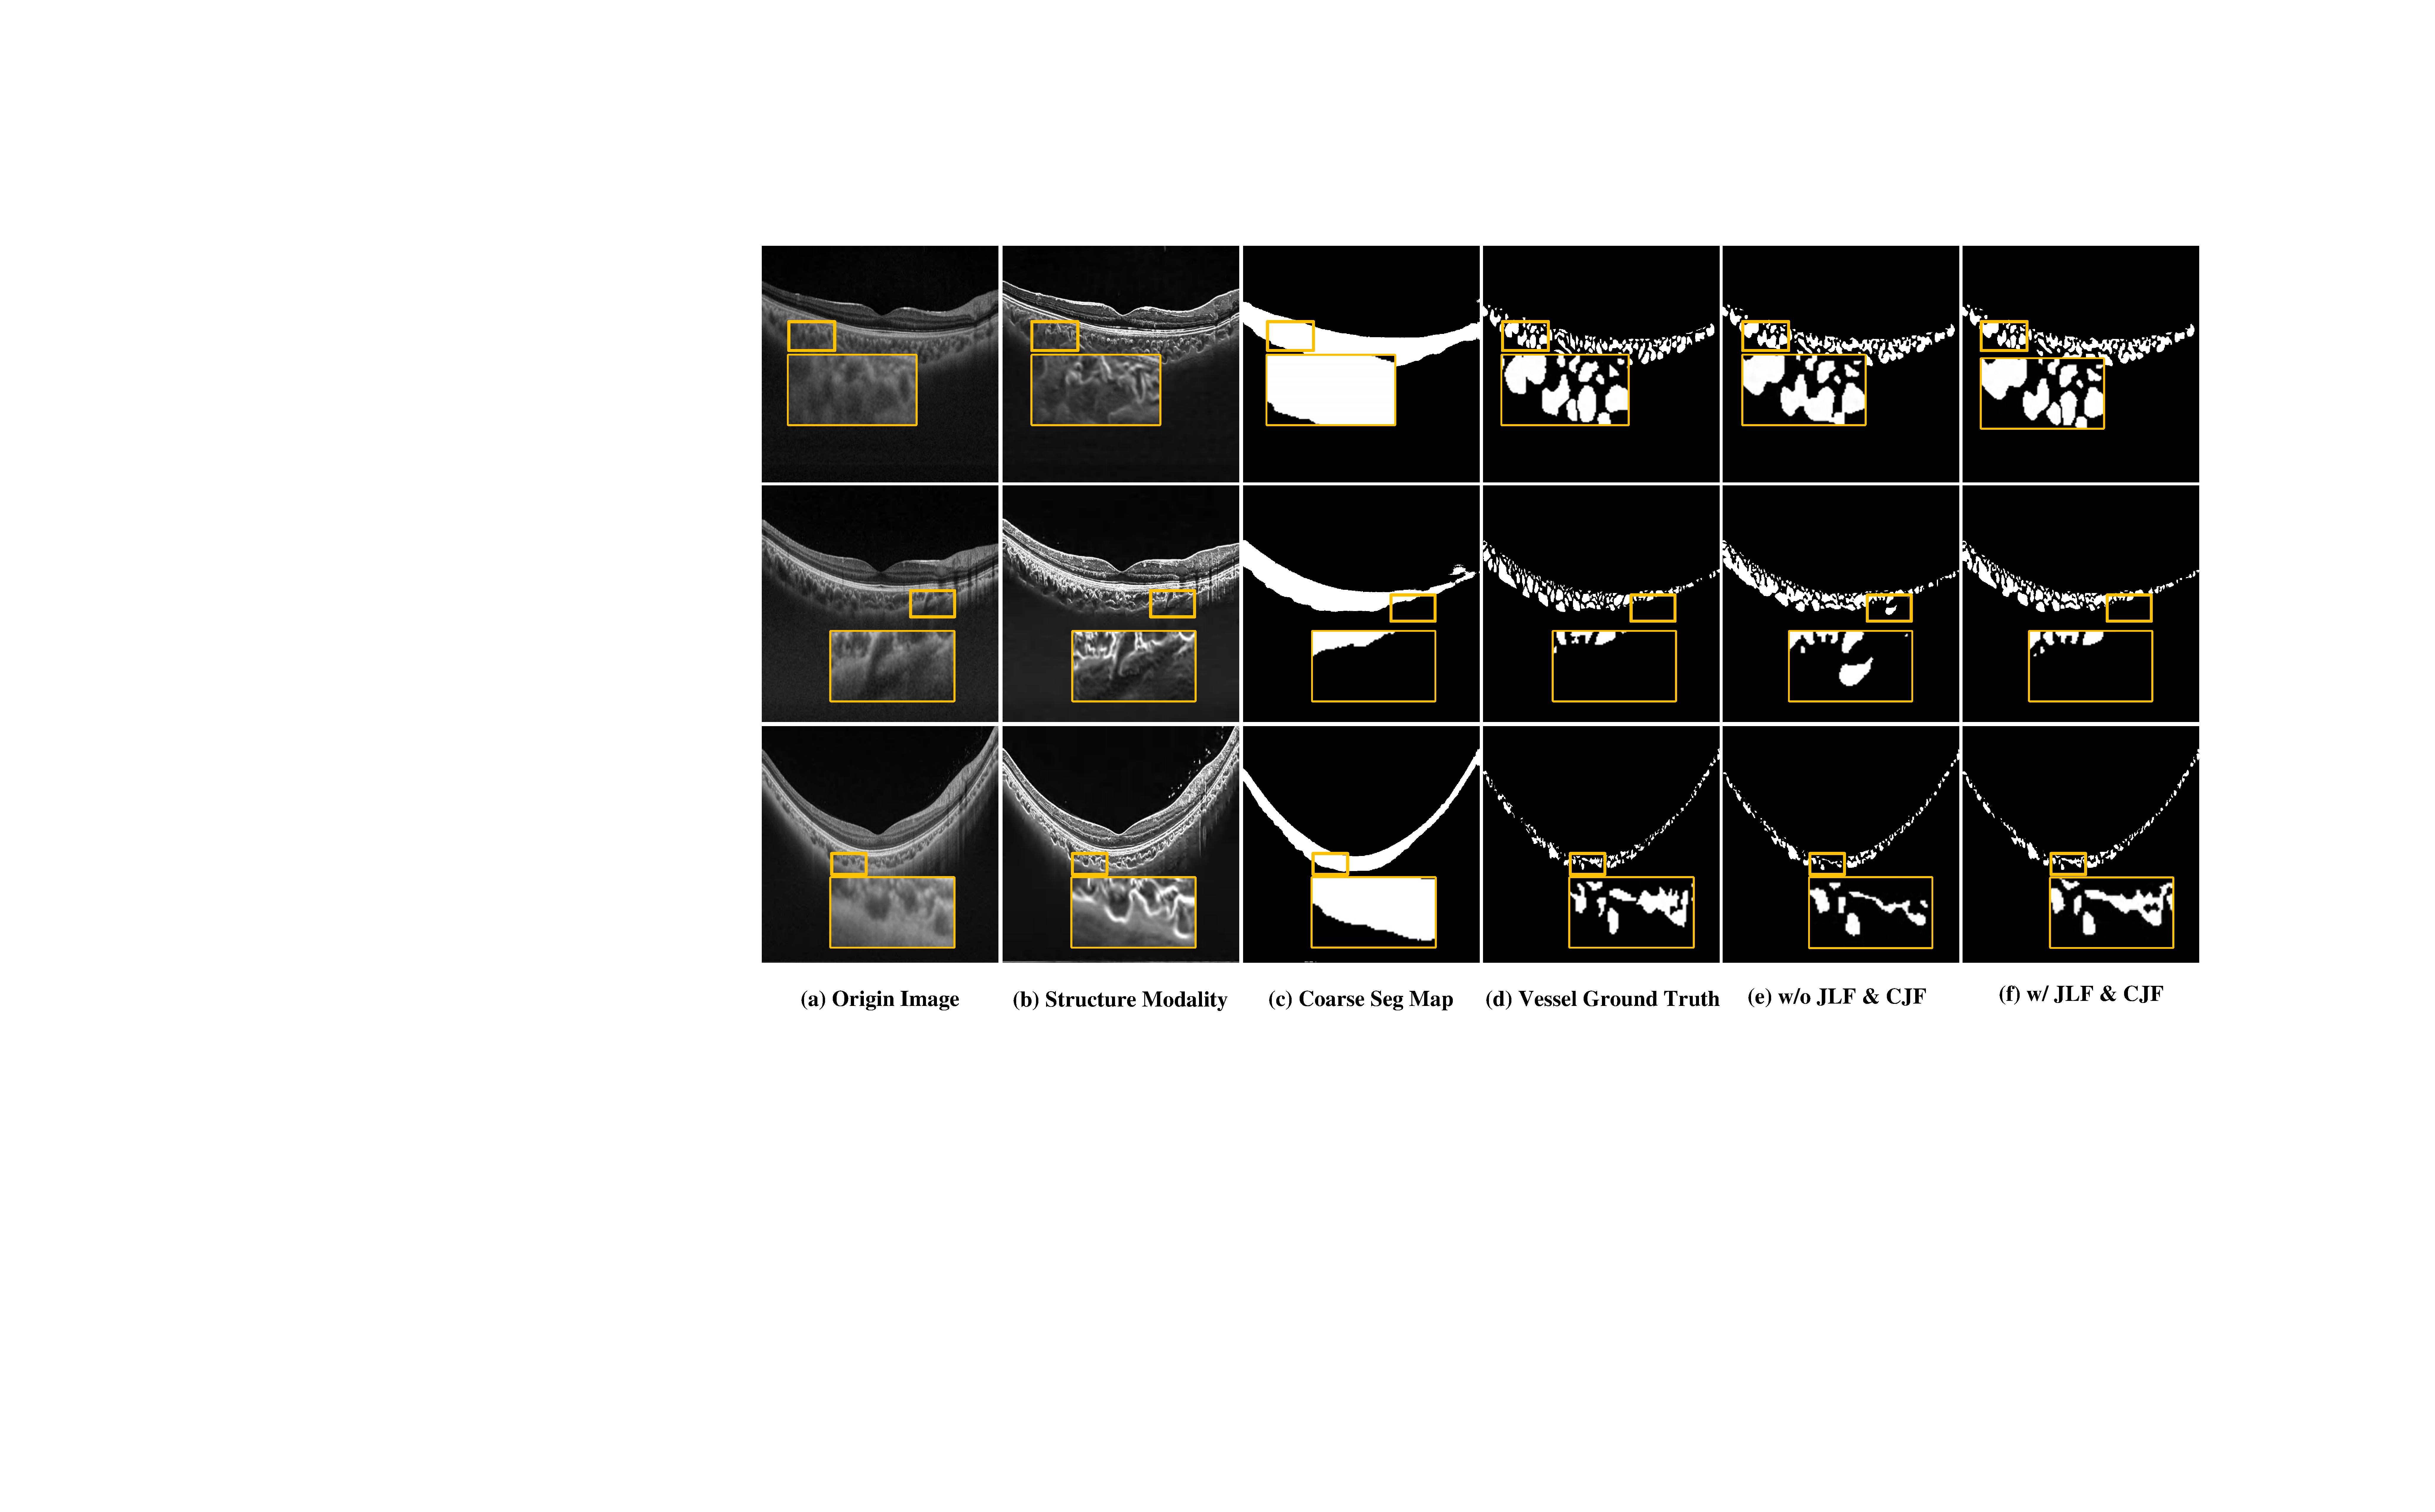
\includegraphics[width=0.6\linewidth]{fig/ablation_jlf_cjf.pdf}
    \caption{Qualitative comparison illustrating the effect of the Joint Loss Function (JLF) and Cascaded Joint Framework (CJF) in SMC-Net.
    (a) Original OCT image, (b) structural prior extracted by UPED, (c) coarse choroidal segmentation, (d) ground truth, (e) prediction without JLF and CJF, and (f) prediction with JLF and CJF.
    The proposed joint modeling effectively suppresses artifacts and improves vessel boundary consistency.}
    \label{fig:ablation_joint_r51}
    \end{figure}


    Specifically, to the best of our knowledge, this is the first work that explicitly formulates choroidal layer segmentation and vessel segmentation as \emph{interdependent tasks within a unified cascaded system}, and systematically analyzes their interaction through both architectural design and loss-level constraints.
    Prior OCT methods typically treat layer segmentation as a preprocessing step or treat vessels independently, without explicitly modeling how layer structure can guide vessel boundaries or how vessel predictions should conform to anatomical layer constraints.
    By contrast, our framework is designed to explore and validate this dependency through a Cascaded Joint Framework (CJF), a joint loss with explicit boundary-level constraints, and structure-aware feature fusion.
    
    From a methodological perspective, each component addresses a specific and well-motivated challenge in choroidal OCT imaging rather than serving as an isolated novelty.
    UPED introduces a noise-robust structural prior to enhance weak and fragmented vessels under severe speckle noise;
    the cascaded design mitigates error accumulation by using the coarse layer prediction as an anatomical region prior rather than a hard segmentation result;
    the joint loss explicitly enforces vessel–layer boundary consistency to suppress anatomically implausible predictions;
    and the SSSD blocks provide linear-complexity long-range modeling to capture the continuity of elongated choroidal vessels, which CNN-based methods struggle with and Transformer-based methods achieve at much higher computational cost.
    Together, these elements form a coherent system tailored to the unique challenges of choroidal vessel segmentation, including error propagation, low-contrast microvasculature, and heavy imaging noise.
    
    Importantly, the novelty of this framework is supported by systematic experimental evidence rather than architectural claims alone.
    As shown in Table~VI, adding UPED to a plain backbone yields only a modest improvement (+1.61\% DSC), whereas the full cascaded joint framework achieves a substantial gain (86.40\% DSC), indicating that the performance improvement arises from explicitly modeling anatomical dependency rather than from any single module.
    Ablation studies further demonstrate that removing the joint loss or the cascaded framework leads to consistent degradation across all metrics, confirming the necessity of the proposed system-level design.
    
    Regarding comparison with recent and state-of-the-art methods, we clarify that our experiments include both domain-specific choroidal segmentation approaches and strong, widely adopted segmentation baselines from the broader medical imaging literature.
    These include CNN-based, Transformer-based, and state-space-based models, ensuring that the reported improvements are not limited to outdated or weak baselines.
    Across both private choroidal datasets and the public RETOUCH benchmark, SMC-Net consistently outperforms recent state-of-the-art methods, supporting the claim of competitive and often superior performance.
    
    Overall, while SMC-Net leverages established building blocks, its contribution lies in proposing and validating a new cascaded joint anatomical modeling paradigm for choroidal OCT segmentation.
    This system-level innovation, together with comprehensive comparisons against recent methods, constitutes the main novelty and practical value of the proposed work.
    For ease of verification, the strengthened ablation analysis and discussion are highlighted in the revised manuscript and quoted below:\\
    \textit{{\color{blue}``\textbf{E. Effectiveness of Joint Anatomical Modeling}\\
    We conduct ablation studies to examine whether explicitly modeling the anatomical dependency between choroidal layers and vessels improves segmentation performance.
    To isolate the effect of the Joint Loss Function (JLF), it is replaced with the Dice--BCE loss, while the Cascaded Joint Framework (CJF) is ablated by removing the pretrained coarse segmentation stage and the choroidal layer decoder in the refinement stage.
    Quantitative results in Table VI (Rows 3--4) demonstrate consistent performance improvements.
    Specifically, JLF improves mIoU, DSC, Acc, Spe, and Sen by 1.60\%, 1.59\%, 0.26\%, 0.32\%, and 1.40\%, respectively, while CJF yields larger gains of 5.40\%, 7.00\%, 0.50\%, 1.50\%, and 12.03\%.
    Qualitative comparisons in Fig.~\ref{fig:ablation_joint_r51} further show that CJF and JLF effectively suppress imaging artifacts and enhance vessel segmentation fidelity.\\
    We further analyze the contribution of UPED relative to architectural components.
    Adding UPED alone to a plain backbone improves vessel DSC from 77.20\% to 78.81\% (+1.61\%), whereas the full SMC-Net configuration (UPED + SSSD + MCAM + SAM + JLF/CJF) achieves 86.40\% DSC.
    Edge ablation results also indicate that UPED outperforms a multi-directional Sobel operator by 2.75\% DSC.
    These results suggest that while UPED provides effective structural priors, the majority of performance gains arise from the proposed joint anatomical modeling, which integrates long-range feature modeling, structure-aware fusion, and boundary-level constraints to fully exploit such priors.
    ''}}
    }\\

    \commentitem The UPED is based on a fixed fractional-differential kernel. While it shows improvement over Sobel, it is not adaptive and cannot learn features from data like a trainable edge detection branch. Its performance depends on the manually chosen fractional order v and the rotation angles. The paper does not mention how the optimal value of v was determined, which maybe a critical hyperparameter.
    
    \commentresponse{2}{
    Thank you for this thoughtful comment regarding the non-adaptive nature of UPED and the role of the fractional-order parameter $v$.
    We agree that it is important to clarify how $v$ is determined and whether it constitutes a critical or sensitive hyperparameter.
    
    In this work, the value of $v$ is selected based on a dedicated sensitivity analysis rather than manual trial-and-error.
    Specifically, we sweep the fractional order over a representative range $v\in\{0.2, 0.4, 0.6, 0.8\}$ on the OCT-CCV validation folds and evaluate the corresponding vessel segmentation performance.
    This range spans from smoother, low-order responses to sharper, higher-order responses, covering the typical operating regime of fractional differential operators.
    For clarity and readability, we summarize the results in Table~\ref{tab:v_sensitivity_1}.
    
    \begin{table}[h]
    \centering
    \caption{Sensitivity analysis of the fractional-order parameter $v$ in UPED on OCT-CCV validation folds.}
    \label{tab:v_sensitivity_1}
    \begin{tabular}{c c c}
    \hline
    $v$ & Vessel DSC (\%) & Qualitative Observation \\
    \hline
    0.2 & 91.42 & Weak vessel edges slightly under-emphasized \\
    0.4 & 91.53 & Stable response, minor attenuation on thin vessels \\
    \textbf{0.6} & \textbf{91.68} & Best balance between edge enhancement and noise suppression \\
    0.8 & 91.39 & Mild noise amplification in low-SNR regions \\
    \hline
    \end{tabular}
    \end{table}
    
    Across the evaluated range, vessel DSC varies by less than 0.3\%, indicating that UPED exhibits low sensitivity to the exact choice of $v$. The best and most consistent performance is achieved at $v=0.6$, which is fixed for all experiments without any dataset-specific tuning.
    Among these settings, $v=0.6$ consistently yields the best average performance and is therefore selected as the default value and fixed for all experiments, without any dataset-specific tuning.
    Lower values ($v=0.2$--$0.4$) slightly under-emphasize weak vessel edges, while higher values (e.g., $v=0.8$) introduce mild noise amplification; however, none of these settings destabilize training or lead to failure cases.
    These observations suggest that $v$ controls a smooth trade-off between edge enhancement and noise amplification rather than acting as a fragile hyperparameter.
    
    Although UPED is not a trainable edge detection branch, this design choice is intentional.
    By using a fixed, theory-grounded fractional-differential operator with a robust operating range, UPED provides a stable and reproducible structural prior that complements data-driven feature learning in the segmentation network.
    In contrast, a fully learnable edge branch would introduce additional trainable parameters and potentially entangle edge extraction with task-specific supervision, which may increase training instability under severe OCT speckle noise.
    
    Regarding orientation parameters, UPED employs a fixed set of four canonical directions ($0^\circ,45^\circ,90^\circ,135^\circ$) and aggregates them into an omni-directional response, eliminating the need for angle tuning.
    Overall, the sensitivity analysis demonstrates that UPED does not rely on carefully tuned hyperparameters; instead, it offers a robust structural prior whose behavior is predictable and easy to reproduce across different OCT imaging conditions.
    
    For transparency, the fractional-order sensitivity analysis has been added to the revised manuscript and is quoted below:\\
    \textit{{\color{blue}``\textbf{C. Fractional-order Sensitivity}\\
    We analyze the sensitivity of the fractional-order parameter $v$ in UPED by sweeping $v\in\{0.2,0.4,0.6,0.8\}$ on the OCT-CCV validation folds.
    Across this range, vessel DSC varies by less than 0.3\%, with the best performance achieved at $v=0.6$, which is fixed for all experiments without dataset-specific tuning.
    Lower values ($v=0.2$--$0.4$) slightly under-emphasize weak vessel edges, while a higher value ($v=0.8$) introduces mild noise amplification; however, none of these settings destabilize training.\\
    UPED employs a fixed set of four canonical orientations ($0^\circ,45^\circ,90^\circ,135^\circ$) and aggregates them into an omni-directional response, eliminating the need for angle tuning.
    These results indicate that UPED exhibits low sensitivity to hyperparameter choices and remains robust and reproducible across varying OCT noise levels and imaging conditions.
    ''}}
    }

    \commentitem The section of A. Pretrained coarse segmentation stage in the “III METHODOLOGY” mainly introduces a unsupervised prior edge detector UPED, which is derived from the Grunwald -Letnikov definition. However, where is a Mamba-based U-shaped network to roughly segment the choroidal layer in this section and how does the U-shape network for coarse segmentation filter artifacts and noise?
    
    \commentresponse{3}{
    Thank you for pointing out this potential confusion in Sec.~III-A.
    We agree that the original presentation may have over-emphasized the derivation of UPED and insufficiently explained the role of the Mamba-based U-shaped network in the coarse segmentation stage.
    We have therefore revised this section to explicitly clarify (i) how the U-shaped network performs coarse choroidal layer segmentation, and (ii) how it contributes to noise and artifact suppression.
    
    The coarse segmentation stage is implemented as a supervised Mamba-based U-shaped encoder--decoder network, denoted as $\varPhi_{\text{Pre}}(\cdot)$, which takes the raw OCT image as input and predicts a coarse choroidal layer mask.
    Similar to standard U-Net-style designs, the encoder progressively aggregates low-level appearance cues and high-level contextual information, while the decoder restores spatial resolution via skip connections.
    By replacing conventional convolutional blocks with Mamba blocks, the encoder captures long-range dependencies along the depth and lateral directions, which are critical for recognizing the globally continuous choroidal layer despite local noise and intensity fluctuations.
    The network is trained to segment the choroidal layer at a coarse level, focusing on correct anatomical localization rather than precise boundary refinement.
    
    Importantly, the output of the coarse network is not used as a final segmentation result but as a region-of-interest (ROI) prior.
    Due to the global contextual modeling and supervised learning of layer structure, the predicted coarse mask tends to cover the entire choroidal region while excluding background tissues, imaging artifacts, and speckle-dominated non-choroidal areas.
    This masking operation effectively suppresses noise and artifacts outside the choroid by setting them to zero in both the raw OCT image and the UPED-derived structural map.
    As a result, the subsequent refinement stage operates only within an anatomically plausible region, substantially reducing false positives caused by background noise and improving training stability.
    
    In summary, the Mamba-based U-shaped coarse segmentation network learns a robust, global localization of the choroidal layer and acts as an anatomical ROI filter, while UPED provides complementary structural edge priors.
    Their combination enables effective noise/artifact suppression and stable coarse-to-fine refinement.
    
    The corresponding clarification has been added to Sec.~III-A of the revised manuscript and is quoted below for convenience: \\
    \textit{{\color{blue}``For an input OCT image $x \in \mathbb{R}^{H \times W \times 3}$, the structural information $s$ is extracted by the proposed unsupervised prior edge detector $\text{UPED}$: $s = \text{UPED}(x)$, $s \in \mathbb{R}^{H \times W \times 3}$. The pretrained coarse segmentation network $\varPhi_{\text{Pre}}(\cdot)$ produces a coarse choroidal mask $m_c = \varPhi_{\text{Pre}}(x)$, which is applied to both the original OCT image $x$ and the extracted structural information $s$ to obtain region-of-interest inputs for the refinement stage:
$x_{\text{masked}} = m_c \cap x, \quad s_{\text{masked}} = m_c \cap s,$ where $x_{\text{masked}}, s_{\text{masked}} \in \mathbb{R}^{H \times W \times 1}$.
By restricting the refinement stage to the predicted choroidal region, the cascaded design effectively suppresses non-choroidal noise and artifacts, enabling the subsequent stage to focus on delineating subtle vascular structures within the choroid.
The masked OCT image and structural information are then fed into the refinement stage.''}}
    }

    \commentitem The manuscript claims to address error propagation from cascade models. However, fractional differential operators are still gradient-based and can be sensitive to the high noise levels present in OCT, and the refinement stage is still dependent on the output of the coarse stage. The manuscript would benefit from a robustness analysis of UPED under varying noise conditions, and how does the SMC-Net denoise?
    
    \commentresponse{4}{
    Thank you for this insightful and technically important comment regarding robustness under severe OCT noise and potential error propagation in cascaded models. We agree that these are central concerns for choroidal vessel segmentation and merit explicit clarification.

    First, we clarify what is meant by ``denoising'' in the proposed framework. SMC-Net does not introduce a standalone denoising module. Instead, robustness to speckle noise and artifacts is achieved through the combination of a noise-aware structural prior (UPED) and anatomy-constrained learning in a coarse-to-fine cascade. The goal is not to remove noise explicitly, but to suppress anatomically implausible responses while preserving weak but consistent vascular structures.

    Regarding the use of a fractional differential operator, although UPED is gradient-based, it differs fundamentally from conventional integer-order operators such as Sobel. The fractional order provides a tunable response that interpolates between low- and high-pass behavior, enabling enhancement of weak vessel boundaries while avoiding the strong noise amplification typical of fixed high-pass filters. In addition, UPED aggregates responses across multiple orientations into an omni-directional magnitude, which further stabilizes edge extraction under speckle-dominated noise.

    To assess robustness under varying noise conditions, we analyze the sensitivity of UPED to its fractional-order parameter. Sweeping $v\in\{0.2,0.4,0.6,0.8\}$ results in less than 0.3\% variation in vessel DSC, and the same value ($v=0.6$) is fixed for all experiments. This low sensitivity indicates that UPED does not require delicate tuning and remains stable across different OCT noise and artifact levels. Moreover, edge-ablation results show that UPED consistently outperforms stronger handcrafted alternatives such as multi-directional Sobel on noisy OCT images, providing empirical evidence of its robustness.

    Concerning cascade error propagation, the refinement stage is not blindly dependent on the coarse output. The coarse mask serves as a conservative anatomical region-of-interest prior that suppresses background noise and non-choroidal artifacts, rather than a hard truncation of fine structures. Importantly, the refinement network still receives the masked raw OCT image and the masked UPED structural cues, allowing it to correct minor boundary inaccuracies from the coarse stage. Empirically, the dominant failure mode of the coarse prediction is slight over-coverage rather than under-segmentation, which provides a safety margin for refinement.

    Overall, robustness in SMC-Net arises from three complementary mechanisms: (i) a stable, noise-aware structural prior (UPED), (ii) anatomical restriction via a coarse region-of-interest mask to suppress artifact-driven false positives, and (iii) structure-aware refinement with long-range modeling and boundary-coupled learning. Together, these design choices mitigate the impact of OCT noise and prevent error amplification in the cascade, explaining the stable performance observed under high-noise conditions.
    }

    \commentitem The multi-stage and multi-module architecture is computationally heavy for both training and inference, with no analysis of efficiency. This complexity analysis would concern about:1)Training Complexity: The need to train (or pre-train) multiple components sequentially or jointly increases the overall training time and complexity. 2)Inference Speed: While the SSSD blocks are designed for efficiency, the full pipeline's inference time is likely higher than single-stage models like U-Net. This could be a barrier to real-time clinical deployment, especially on resource-constrained hardware. A comparison of inference time (FPS) or number of FLOPs against other models is absent. 3)Parameter Count: The paper introduces Tiny, Small, and Base variants but only reports the performance of the best one (SMC-Net-S) in the main comparison. The performance and efficiency trade-offs of these variants are not discussed.\\
    \commentresponse{5}{
    We sincerely thank the reviewer for raising this important and practical concern regarding computational efficiency and clinical viability. We fully agree that, for a multi-stage framework to be convincing, it must be accompanied by transparent evidence on model complexity, inference latency, and accuracy--efficiency trade-offs.
    \begin{table}[!h]
    \renewcommand{\arraystretch}{1.15}
    \centering
    \begingroup\color{blue}\small
    \setlength{\tabcolsep}{4pt}
    \captionsetup[table]{name=Table III.}{Table III: Inference-time breakdown of the SMC-Net series on OCT-CCV ($512\times512$, fp32, batch=1) on an RTX 4090 D. SMC-Net-S is measured; SMC-Net-T/B are estimated by scaling the measured network time (coarse+refine) linearly with GFLOPs while keeping UPED fixed at $0.8$~ms.}
    \label{tab:inference_time_smcnet_r55}
    \resizebox{0.7\linewidth}{!}{
    \begin{tabular}{@{}lcccccc@{}}
    \toprule
    Variant & Params (M) & GFLOPs (G) & UPED (ms) & Coarse+Refine (ms) & Total (ms) & FPS \\ \midrule
    SMC-Net-T & 11.14 & 17.60 & 0.8 & 3.1 & 3.9 & 257 \\
    SMC-Net-S & 49.04 & 67.18 & 0.8 & 11.8 & 12.6 & 79 \\
    SMC-Net-B & 72.89 & 195.73 & 0.8 & 34.4 & 35.2 & 28 \\ \bottomrule
    \end{tabular}
    }
    \endgroup
    \end{table}
    \setcounter{figure}{6}
    \begin{figure}[h]
    \centering
    \begingroup\color{blue}
    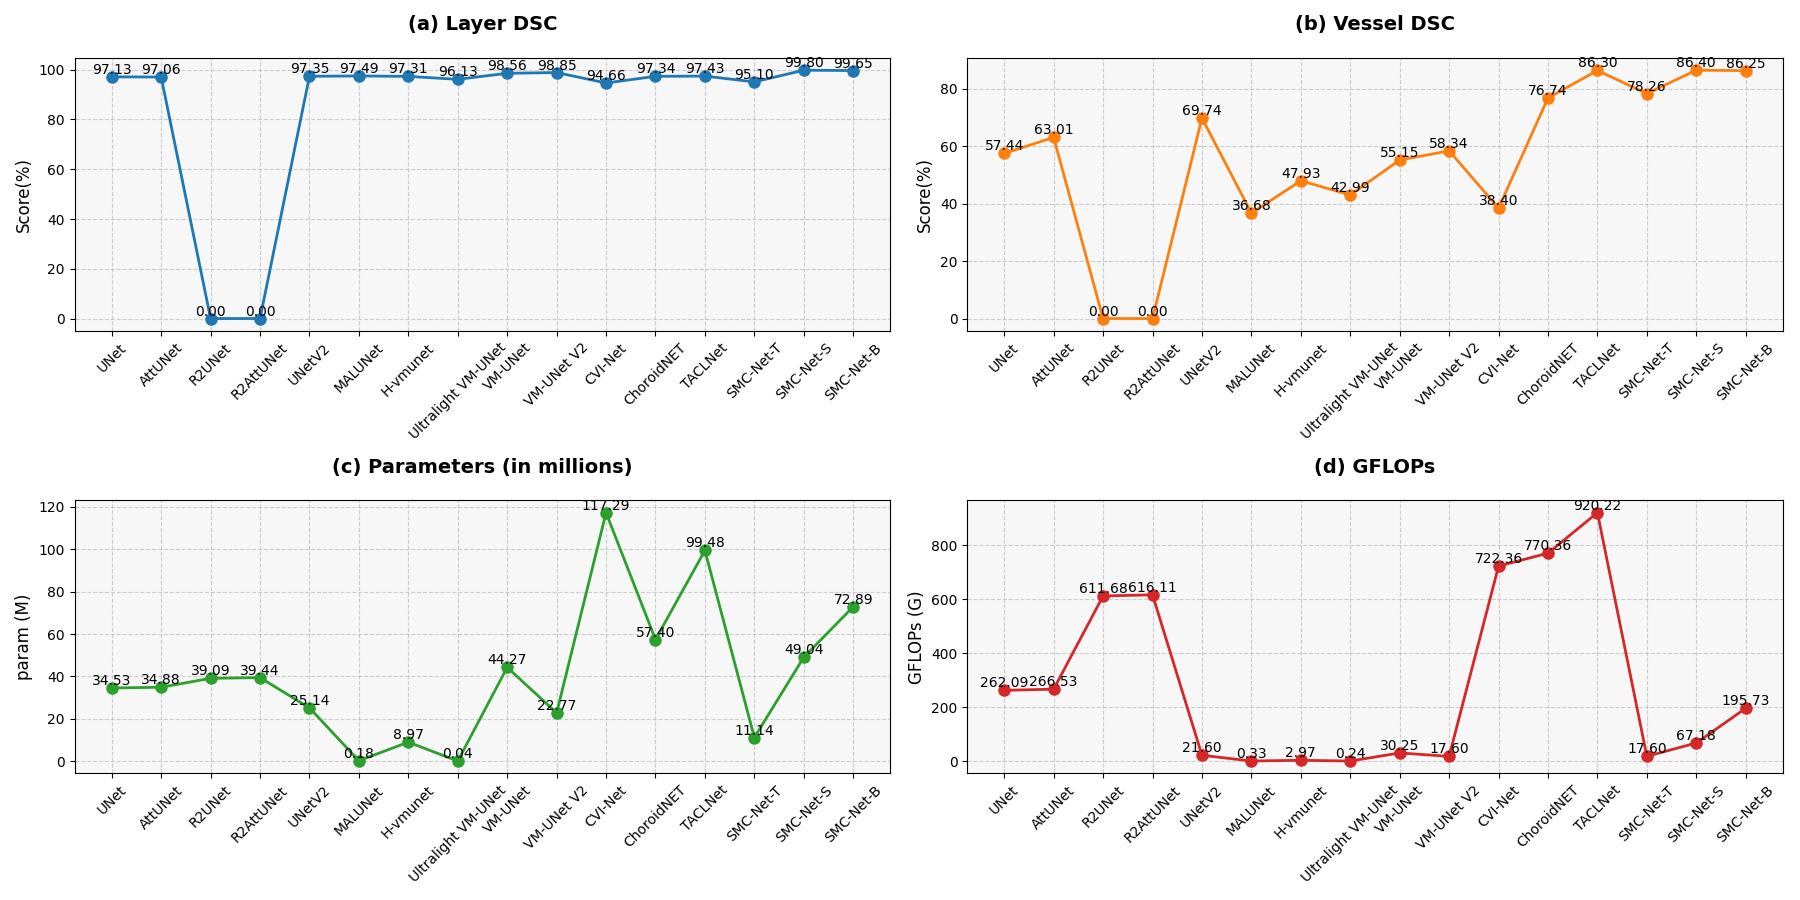
\includegraphics[width=0.9\linewidth]{fig/complexity_compare.png}
    \caption{Accuracy--efficiency trade-off on OCT-CCV ($512\times512$, batch=1, fp32). (a) Layer DSC, (b) Vessel DSC, (c) Params (M), (d) GFLOPs (G).}
    \label{fig:complexity_compare_r55}
    \endgroup
    \end{figure}\\
    To address this, we provide a systematic analysis of computational cost and performance in the Ablation Studies section. First, we report parameter count and GFLOPs across different model scales (Tiny, Small, and Base) and compare them with representative baselines. As shown in Fig.~\ref{fig:complexity_compare_r55}, the proposed SMC-Net series consistently achieves a favorable accuracy--efficiency trade-off. In particular, SMC-Net-S attains the best choroidal layer and vessel DSC while maintaining moderate model size (49.04M parameters) and computational cost (67.18 GFLOPs). Compared with the Transformer-based TACLNet, SMC-Net-S achieves comparable or better performance with approximately half the parameters and nearly one order of magnitude fewer GFLOPs, highlighting its efficiency advantage.

    Second, we explicitly report inference latency in Sec.V-A-2~\emph{Inference Time}. On a single NVIDIA RTX 4090 D GPU (fp32, batch size 1, $512\times512$ input), SMC-Net-S processes one OCT image in 12.6~ms (approximately 79 FPS), demonstrating suitability for real-time or near-real-time deployment. Table III further provides a detailed breakdown of inference time, separating the cost of the UPED module from the coarse and refinement stages, and shows consistent scaling behavior across model variants.

    Together, these results provide a transparent view of the computational characteristics of SMC-Net, including FLOPs, parameter count (as a proxy for memory footprint), and inference latency, and substantiate the claim that the proposed framework achieves a strong balance between segmentation accuracy and computational efficiency suitable for practical and resource-constrained clinical settings.
    
    The newly clarified efficiency text is highlighted in the revised manuscript and is quoted below in italics for convenience:\\
    \textit{{\color{blue}``\textbf{A. Scaling Trends of Computational Complexity and Performance}\\ \textbf{1) Architecture and FLOPs Scaling}\\ In addition to segmentation accuracy, we compare model complexity in terms of parameter count and GFLOPs on the OCT-CCV dataset. As shown in Fig.~\ref{fig:complexity_compare_3}, the proposed SMC-Net series consistently achieves a favorable accuracy--efficiency trade-off. In particular, SMC-Net-S attains the best choroidal layer and vessel DSC while maintaining moderate model size and computational cost.\\ \textbf{2) Inference Time}\\ We further evaluate inference efficiency on a single NVIDIA RTX 4090 D GPU (batch size 1, $512\times512$, fp32). SMC-Net-S processes one OCT image in 12.6~ms (approximately 79 FPS), demonstrating its suitability for real-time or near-real-time deployment. Table III reports the inference-time breakdown of the SMC-Net series, showing consistent scaling behavior across Tiny, Small, and Base variants.Compared with the Transformer-based TACLNet~\cite{wen2024}, SMC-Net-S achieves comparable or better performance with approximately half the parameters and nearly one order of magnitude fewer GFLOPs. Moreover, performance gains saturate beyond SMC-Net-S (49.04M parameters), indicating diminishing returns from further model scaling.''}}\\
    }

    \commentitem The manuscript designed the Structure Aware Module (see Fig. 4) to merge structure features and semantics during the Structure-Aware Phase. What is the semantics?
	    
    \commentresponse{6}{
    Thank you for this clarification request regarding the term ``semantics'' in the Structure-Aware Module (SAM). We agree that this concept should be stated more explicitly.

    Many works refer to the deep features of neural networks as semantic features, because these features are used to perform semantic understanding tasks such as classification and segmentation. In our framework, ``semantic features'' refer to the high-level feature representations produced by the OCT encoder in the refinement stage. These features encode contextual and categorical information learned from data, such as vessel presence, surrounding tissue appearance, and layer-level context, rather than explicit geometric or boundary information. Their role is to infer \emph{what} anatomical structure a pixel most likely belongs to, based on appearance and contextual cues.

    In contrast, the UPED-derived structural features explicitly encode \emph{where} intensity transitions and topology-consistent boundaries occur, which are particularly important for delineating weak and thin choroidal vessels under severe speckle noise. The role of SAM is therefore to inject these explicit structural cues into the semantic feature space via channel-wise and spatial attention, so that high-level semantic representations become more boundary-aware and anatomically consistent.

    In summary, the ``semantics'' in SAM correspond to learned, high-level OCT feature representations from the encoder, while the structural cues come from UPED. SAM bridges these two types of information to improve vessel boundary localization and robustness.
    }

    \commentitem The manuscript proposed a structure-aware dual-branch network to jointly model features from both the choroid layer and vessels, explicitly capturing their anatomical relationships for precise segmentation. What are their anatomical relationships between choroid layer and vessels, and why can the structure-aware dual-branch network capture it?
    
    \commentresponse{7}{
    Thank you for this important question regarding the anatomical motivation behind the proposed structure-aware dual-branch network. We agree that explicitly clarifying the anatomical relationship between the choroidal layer and vessels, as well as how it is captured by the network, is essential.

    From an anatomical perspective, choroidal vessels are not isolated structures but are embedded within and constrained by the choroidal layer. Their spatial distribution, continuity, and visibility are strongly governed by the extent and thickness of the choroid: vessels reside exclusively within the choroidal region, follow its elongated geometry, and often weaken or disappear near layer boundaries. Consequently, errors in identifying the choroidal layer (e.g., leakage beyond the layer or truncation within it) directly translate into anatomically implausible vessel predictions.

    The proposed structure-aware dual-branch network is designed to explicitly model this dependency. One branch focuses on capturing coarse-to-fine representations of the choroidal layer, providing global anatomical context and a spatially valid region of interest. The other branch focuses on vessel segmentation, emphasizing fine-grained and weak vascular structures. Structural cues derived from UPED are injected into semantic feature representations via the Structure-Aware Module (SAM), enabling vessel features to be refined under explicit awareness of layer boundaries.

    Furthermore, the Cascaded Joint Framework and the joint loss function explicitly couple the predictions of the two branches at the boundary level. This design encourages vessel predictions to be anatomically consistent with the choroidal layer, suppressing false positives outside the layer and reinforcing continuity within it. Through joint feature fusion and boundary-level constraints, the network learns not only appearance-based cues but also the inherent anatomical relationship between layers and vessels.

    In summary, the anatomical relationship is that choroidal vessels are spatially constrained and structurally dependent on the choroidal layer. The structure-aware dual-branch design captures this relationship by combining global layer context, structure-aware feature fusion, and explicit joint constraints, leading to more anatomically consistent and precise segmentation.
    }

    \commentitem The coarse segmentation and fine-grained segmentation methods basically use similar loss functions for training. What different results do these two networks learn, and why do you adopt this approach?
    
    \commentresponse{8}{
    Thank you for this insightful question regarding the use of similar loss functions in the coarse and refinement stages.
    We agree that it is important to clarify what different outcomes these two networks are optimized to learn and why this design is adopted.
    
    Although both stages involve Dice--BCE–based terms, they are trained under different loss formulations and supervision scopes, leading to fundamentally different learning objectives.
    As defined in Eq.~(8), the coarse segmentation stage is optimized using
    $L_{\text{coarse}} = L_{\text{Dice}} + L_{\text{BCE}}$,
    where the supervision target is only the choroidal layer mask.
    This loss encourages high overlap between prediction and ground truth at a region level, without imposing any constraints on boundary sharpness or vessel-related structures.
    As a result, the coarse network learns to robustly localize the entire choroidal region and suppress background noise and artifacts, producing a conservative region-of-interest mask rather than a precise anatomical delineation.
    
    In contrast, the refinement stage is optimized using the joint loss in Eq.~(9),
    \[
    L_{\text{joint}} = L_{\text{DiceBCE}}(y_v,\hat{y}_v) + L_{\text{DiceBCE}}(y_l,\hat{y}_l) + \frac{1}{N}\sum_{i=1}^{N}(y_{\text{inter}} - \hat{y}_v)^2,
    \]
    which simultaneously supervises vessel segmentation ($y_v$) and choroidal layer segmentation ($y_l$) while explicitly enforcing their anatomical relationship.
    The additional intersection penalty term constrains vessel predictions to lie within the predicted choroidal layer, directly coupling fine-grained vessel boundaries with layer boundaries.
    Consequently, the refinement network is driven to learn sharp vessel structures, accurate boundaries, and anatomically consistent vessel--layer interactions, which are not required or encouraged by the coarse loss.
    
    We adopt this two-stage design because it separates learning objectives according to task difficulty and anatomical relevance.
    The coarse stage uses a simple and robust loss to learn stable global localization under severe OCT noise, minimizing the risk of error amplification.
    The refinement stage then leverages a more structured joint loss to learn fine-grained, anatomy-aware segmentation within a restricted and anatomically plausible region.
    Although both stages share Dice--BCE components for optimization stability, the presence or absence of vessel supervision and anatomical constraints leads them to learn qualitatively different results.
    }
	\end{enumerate}

\nocite{*}
\bibliographystyle{IEEEtran}
\bibliography{reference}

\end{document}
